%
% File acl2021.tex
%
%% Based on the style files for EMNLP 2020, which were
%% Based on the style files for ACL 2020, which were
%% Based on the style files for ACL 2018, NAACL 2018/19, which were
%% Based on the style files for ACL-2015, with some improvements
%%  taken from the NAACL-2016 style
%% Based on the style files for ACL-2014, which were, in turn,
%% based on ACL-2013, ACL-2012, ACL-2011, ACL-2010, ACL-IJCNLP-2009,
%% EACL-2009, IJCNLP-2008...
%% Based on the style files for EACL 2006 by 
%%e.agirre@ehu.es or Sergi.Balari@uab.es
%% and that of ACL 08 by Joakim Nivre and Noah Smith

\documentclass[11pt,a4paper]{article}
\usepackage[hyperref]{acl2021}
\usepackage{times}
\usepackage{latexsym}
\usepackage{graphicx}
\usepackage{CJKutf8}
\usepackage{amsmath}
\usepackage{bm}
\usepackage{booktabs}
\usepackage{multirow}
\usepackage{url}
\usepackage{breakurl}

% ADD FOR PICT
\usepackage{tikz-dependency}
\usepackage{amsmath}
\usepackage{graphicx}
\usepackage{pgfplots}
\usepackage{tikz}
\usepackage[center]{subfigure}
\usepackage{tikz-qtree}
\usepgflibrary{arrows.meta}
\usepgfplotslibrary{fillbetween}
\usetikzlibrary{fit, calc, decorations.pathreplacing, positioning, shapes.geometric, backgrounds}
\usepackage{float}
% ADD FOR PICT END

\def\UrlBreaks{\do\/\do-}

\renewcommand{\UrlFont}{\ttfamily\small}

% This is not strictly necessary, and may be commented out,
% but it will improve the layout of the manuscript,
% and will typically save some space.
\usepackage{microtype}

\aclfinalcopy % Uncomment this line for the final submission
\def\aclpaperid{2185} %  Enter the acl Paper ID here

%\setlength\titlebox{5cm}
% You can expand the titlebox if you need extra space
% to show all the authors. Please do not make the titlebox
% smaller than 5cm (the original size); we will check this
% in the camera-ready version and ask you to change it back.

\newcommand\BibTeX{B\textsc{ib}\TeX}

\title{
%An In-depth 
% Study on Deep Syntactic Char-level Structures of Chinese Words
% An In-depth Study on Char-level Syntactic Structure of Chinese Words
An In-depth Study on Internal Structure of Chinese Words
}

\author{
Chen Gong$^{1}$, Saihao Huang$^1$\thanks{$~$ Chen Gong and Saihao Huang make equal contributions to this
work. Zhenghua is the corresponding author.}, Houquan Zhou$^1$, Zhenghua Li$^1$, Min Zhang$^1$,\\ {\bf Zhefeng Wang}$^2$, {\bf Baoxing Huai}$^2$, {\bf Nicholas Jing Yuan}$^2$ \\
$^1$Institute of Artificial Intelligence, School of Computer Science and Technology, \\Soochow University, China; $~~~~~$
$^2$ Huawei Cloud, China  \\
{\tt $^1$\{cgong,shhuang1999,hqzhou\}@stu.suda.edu.cn} \\
{\tt $^1$\{zhli13,minzhang\}@suda.edu.cn} \\
{\tt $^2$\{wangzhefeng, huaibaoxing, nicholas.yuan\}@huawei.com} \\
}


\date{}

\begin{document}
\maketitle
\begin{CJK}{UTF8}{gkai}
\begin{abstract}
\label{sec:abstract}

%% 1. what is the problem 
Scientific applications that run on leadership computing facilities often face the challenge 
of being unable to fit leading science cases onto accelerator devices due to memory constraints 
(memory-bound applications).
%
% 2. what is your solution 
In this work, the authors studied one such US Department of Energy mission-critical condensed matter 
physics application, Dynamical Cluster Approximation (DCA++), and this paper discusses how device memory-bound challenges were successfully reduced  by proposing an effective 
``all-to-all'' communication method---a ring communication algorithm. 
%
This implementation takes advantage of acceleration on GPUs and remote direct memory access (RDMA) for fast data exchange between GPUs. 
%
\\Additionally, the ring algorithm was optimized with sub-ring communicators
and multi-threaded support to further reduce communication overhead and 
expose more concurrency, respectively.
%
% 3. What's the cherry-picked evaluation result you want to mention
The computation and communication were also analyzed 
by using the Autonomic Performance Environment for Exascale 
(APEX) profiling tool,  and this paper further discusses the 
performance trade-off for the ring algorithm implementation. 
%
The memory analysis on the ring algorithm shows that the allocation size for the authors' most 
memory-intensive data structure per GPU is now reduced to $1/p$ of the original size, where $p$ is the number of GPUs in the ring communicator.
%
The communication analysis suggests that 
the distributed Quantum Monte Carlo execution time grows linearly as sub-ring size increases, and the cost of messages passing through the network interface connector could be a limiting factor.


%
% \todoRed{Ronnie: Next sentence needs rewrite, too much information about Green's function that no one knows in the abstract; recommend generalizing.} \emph {However, DCA++ is currently facing memory-bound challenge as 
% a larger device array $G_t$ is limited by device memory size, where
% $G_t$ is a two-particle Green's function that allows condensed matter
% scientists to explore larger and more complex (higher fidelity)
% physics cases.}

\end{abstract}

\keywords{DCA++, Quantum Monte Carlo, GPU Remote Direct Memory Access, memory-bound issue, exascale machines}

\section{Introduction}  \label{sec:introduction}

\newcommand\inexpIntro[3]{#1?(#2,#3).}
\newcommand\rinexpIntro[3]{*#1?(#2,#3).}
\newcommand\outexpIntro[3]{#1!(#2,#3).}
\newcommand\outatomIntro[3]{#1!(#2,#3)}

We propose a fully automated method for proving termination of \(\pi\)-calculus processes.
Although there have been a lot of studies on termination analysis for the \(\pi\)-calculus
and related calculi~\cite{Deng06IC,Demangeon07,SangiorgiTermination,KobayashiHybrid,Yoshida04IC,DBLP:journals/jlp/DemangeonHS10,Venet98SAS}, most of them have been rather theoretical,
and there have been surprisingly little efforts in developing  fully automated termination
verification methods and tools based on them. To our knowledge,
Kobayashi's \typical{}~\cite{TyPiCal,KobayashiHybrid} is the only exception that
can prove termination of \(\pi\)-calculus processes (extended with natural numbers)
fully automatically, but its termination analysis is quite limited (see Section~\ref{sec:relatedwork}).

Our method is based on a reduction to termination analysis for sequential programs:
we translate a \(\pi\)-calculus process \(P\) to a sequential program \(S_P\), so that
if \(S_P\) is terminating, so is \(P\). The reduction allows us to use
powerful, mature methods and tools
for termination analysis of sequential programs~\cite{heizmann2016ultimate,freqterm,DBLP:conf/lics/PodelskiR04,Kuwahara2014Termination,DBLP:journals/cacm/CookPR11}.

The idea of the translation is to convert a chain of communications on replicated input
channels to a chain of recursive function calls of the target sequential program.
Let us consider the following Fibonacci process:
\begin{align*}
    & \rinexpIntro{\fib}{n}{r}
        \ifexp{n<2}{ \soutatom{r}{1} \\ &\quad}
                   { \nuexp{s_1} \nuexp{s_2} (\outatomIntro{\fib}{n-1}{s_1} \PAR \outatomIntro{\fib}{n-2}{s_2} \PAR \sinexp{s_1}{x}\sinexp{s_2}{y}\soutatom{r}{x+y}) \\}
    & \PAR \outatomIntro{\fib}{m}{r}
\end{align*}
Here, the process
$\rinexpIntro{\fib}{n}{r} \ldots$ is a function server that computes the \(n\)-th Fibonacci number
in parallel and returns the result to \(r\),
and $\outatom{\fib}{m}{r}$ sends a request for computing the \(m\)-th Fibonacci number;
those who are not familiar with the syntax of the \(\pi\)-calculus may wish to consult
Section~\ref{sec:targetlanguage} first.
To prove that the process above is terminating for any integer \(m\),
it suffices to show that there is no infinite chain of communications on $\fib$:
\[
    \fib(m,r) \to \fib(m_1,r_1) \to \fib(m_2,r_2) \to \cdots.
\]
We convert the process above to the following program:\footnote{The actual translation
  given later is a little more complex.}
\begin{verbatim}
 let rec fib(n) = if n<2 then () else (fib(n-1) [] fib(n-2)) in
 fib(m)
\end{verbatim}
Here, \texttt{[]} represents the non-deterministic choice.
Note that, although the calculation of Fibonacci numbers is not preserved,
for each chain of communications on \texttt{fib}, there is a corresponding
sequence of recursive calls:
\[
\mathtt{fib}(m) \to \mathtt{fib}(m_1) \to \mathtt{fib}(m_2) \to \cdots.
\]
Thus, the termination of the sequential program above implies the termination of
the original process.
As shown in the example above, (i) each communication on a replicated input channel
is converted to a function call, (ii) each communication on a non-replicated input
channel is just removed (or, in the actual translation, replaced by a call of
a trivial function defined by \(f(\seq{x})=(\,)\)), and (iii) parallel composition
is replaced by a non-deterministic choice.
We formalize the translation outlined above and prove its correctness.

The basic translation sketched above sometimes loses too much information.
For example, consider the following process:
\begin{align*}
    & \rinexpIntro{\pre}{n}{r} \soutatom{r}{n-1} \\
    & \PAR \rinexpIntro{f}{n}{r} \ifexp{n<0}{ \soutatom{r}{1} }
                                       { \nuexp{s} (\outatomIntro{\pre}{n}{s} \PAR \sinexp{s}{x}\outatomIntro{f}{x}{r}) } \\
    & \PAR \outatomIntro{f}{m}{r}
\end{align*}
The translation sketched above would yield:
\begin{verbatim}
  let pred(n) = n-1 in
  let rec f(n) = if n<0 then () else (pred(n) [] f(*)) in
  f(m)
\end{verbatim}
Here, \texttt{*} represents a non-deterministic integer: since we have removed
the input $\sinatom{s}{x}$, we do not have information about the value of \( x \).
As a result, the sequential program above is non-terminating, although the original
process is terminating.
To remedy this problem, we also refine the basic translation above by using a refinement
type system for the \(\pi\)-calculus. Using the refinement type system,
we can infer that the value of \(x\) in the original process is less than \(n\),
so that we can refine the definition of \texttt{f} to:
\begin{verbatim}
 let rec f(n) = ... else (pred(n) [] let x=* in assume(x<n);f(x))
\end{verbatim}
The target program is now terminating, from which
we can deduce that the original process is also terminating.
We have implemented an automated tool based on the refined translation above.

The contributions of this paper are summarized as follows.
\begin{itemize}
\item The formalization of the basic translation from the \(\pi\)-calculus
  (extended with integers) to sequential programs, and a proof of its correctness.
\item The formalization of a refined translation based on a refinement type system.
\item An implementation of the refined translation, including automated refinement type
  inference based on CHC solving, and experiments to evaluate the effectiveness of
  our method.
\end{itemize}

The rest of this paper is structured as follows.
Section~\ref{sec:targetlanguage} introduces the source and target languages
of our translation.
Section~\ref{sec:approach} 
formalizes the basic translation, and proves its correctness.
Section~\ref{sec:refinement} refines the basic translation by using a refinement type system.
Section~\ref{sec:implementation} reports an implementation and experiments.
Section~\ref{sec:relatedwork} discusses related work,
and Section~\ref{sec:conclusion} concludes the paper.

\textbf{Related work}:
% Object detection related datasets/algo in non-medical domain
% Locally labeled CXR dataset
A few CXR datasets have localized abnormality annotations \cite{shih2019augmenting,filice2020crowdsourcing,jaeger2014two} that are curated manually. These are high quality gold standard ground truth datasets but tend to be smaller in scale (< 30,000 images) and have a narrow coverage, with typically only 1-2 labels. In addition, since most labeling efforts only have abnormality semantics attached, no direct relationships with the affected anatomical locations are available. 

%MEHDI: repeated concepts from above. I am removing the following: 

%The lack of anatomic semantics in the annotation is a limitation for complex multi-modal clinical reasoning work, e.g., differential diagnosis, since clinicians often integrate information along anatomical lines, and for downstream report generation tasks, which often requires describing not only the abnormality but also correctly communicate the location of the abnormalities (and medical devices) to the receiving clinicians. 

Two recent CXR datasets have labels for anatomies described in the reports. In \cite{datta2020dataset}, a small manually annotated dataset (2000 reports) included 10 abnormalities that are individually associated with 29 unique spatial locations (anatomies) at the report level. Another CXR dataset has automatically extracted abnormality and anatomy labels as disconnected concepts that are only correlated at the study level from  160,000 reports using a supervised NLP algorithm \cite{bustos2020padchest}. This was trained on a smaller set of manually annotated data. Neither datasets contain localized annotations for the associated CXR images, nor any comparison relation annotations between sequential exams, both of which are available in the Chest ImaGenome dataset. In Table \ref{tab:related}, we present a comparison of our Chest ImagGenome dataset with other datasets available in the literature.

% Table -- Kashyap

% MEdical imaging datasets to go here: Discussed that we will only focus on cxr datasets that are available for this paper. 
% \caption{\color{red} Kashyap, feel free to continue with the table. We should remove the questionmarks and add a line for our dataset (since all others are not graph). For longer text, using abbreviations and explaining them in the caption often works better. If fill in the values is not possible, it is better to remove the table altogether.}


\begin{table}[t!]
\caption{Summary of existing chest X-ray datasets}
\resizebox{\textwidth}{!}{%
\begin{tabular}{@{}lllllllll@{}}
\toprule
\textbf{Dataset} & \textbf{Annotation Level} & \textbf{Annotation Method} & \textbf{Num Labels} & \textbf{Anatomy Labeled} & \textbf{Graph} & \textbf{Dataset Size} & \textbf{Temporal Labels} & \textbf{Reports} \\ \midrule
SIIM-ACR Pneumothorax Segmentation \cite{filice2020crowdsourcing} & Segmentation & Manual + augmented & 1 & No & No & 12,047 & No & No \\
RSNA Pneumonia Detection Challenge   \cite{shih2019augmenting} & Bounding Boxes & Manual & 1 & No & No & 30,000 & No & No \\
Indiana University Chest X-ray collection \cite{demner2016preparing} & Global & Automated & 10 & No & No & 3,813 & No & Yes \\
NIH CXR dataset \cite{wang2017chestx} & Global & Automated & 14 & No & No & 112,120 & No & No \\
PLCO \cite{team2000prostate} & Global & Automated & 24 & Yes & No & 236,000 & Yes & No \\
Stanford CheXpert \cite{irvin2019chexpert} & Global & Automated & 14 & No & No & 224,316 & No & No \\
MIMIC-CXR \cite{johnson2019mimic} & Global & Automated & 14 & No & No & 377,110 & No & Yes \\
Dutta \cite{datta2020dataset} & Global & Manual & 10 & Yes & Yes & 2,000 & No & Yes \\
PadChest \cite{bustos2020padchest} & Global & Manual + automated & 297 & Yes & No & 160,868 & No & Yes \\
Montgomery County Chest X-ray   \cite{jaeger2014two} & Segmentation & Manual & 1 & Yes & No & 138 & No & No \\
Shenzen Hospital Chest X-ray   \cite{jaeger2014two} & Segmentation & Manual & 1 & Yes & No & 662 & No & No \\  \hline \hline
\textbf{Chest ImaGenome} & Bounding Boxes & Automated & 131 & Yes & Yes & 242,072 & Yes & Yes \\
\bottomrule
\end{tabular}%
}
\label{tab:related}
\vspace{-0.4cm}
\end{table}
% removed (Derived from MIMIC-CXR \cite{johnson2019mimic}) % makes table really small



\section{Word-internal Structure Annotation}\label{sec:data-annotation}
%Intra-Word Character Dependency Treebank (IWDT)}

In this section, we describe in detail the annotation process of WIST. 
As shown in Figure \ref{fig:example}-(c), we adopt dependency trees for representing word-internal structure. 
The reason is two-fold. First, word-formation process correlates with syntax in different ways depending on language type \cite{Aikhenvald-2007-typological}. Such correlation is especially close for Chinese due to its lack of morphological inflections. In particular, \citet{grammar-notes-zhu-1982} presented thorough  investigation on Chinese word formation mainly from a syntactic view. 
Second, as a grammar formalism, dependency tree structure has been widely adopted for capturing sentence-level syntax due to its simplicity and flexibility in representing  relations. Meanwhile, its computational modeling is also developed quite well. 
%我们为什么采用依存树的形式?首先,汉语词内部结构本身和句法紧密相关,给出参考文献。第二,依存句法树形式,是近年来最流行的句法表示方法,多语言使用。主要就在于可以用label来区分组合的模式。




% 传统的人工标注数据通常以词为基本的syntactic unit, such as CTB, PKU, MSR, 
% This form of annotation does not
% give character-level syntactic structures for words,
% a source of linguistic information that is more fundamental
% and less sparse than atomic words.

% Considering that a word is defined by all the characters inside that subtly interact with each other from both syntax and semantics.
% Unlike alphabetical languages, Chinese
% characters convey meanings, and the meaning of
% most Chinese words takes roots in their character.a series of work因此一些工作开始标注词内部结构【引用】。most of the previous annotations通常只考虑内部结构框架或者核心字的位置,忽略了词内部各constituent unit之间的关系。Zhao 通过combine character-level POS tag来表示dependency label.然而这种表示不能直观地展示出各个字直接的主谓宾定状补关系。
% To overcome this obstacle, we construct一个词内部结构数据集according to our newly complied annotation guideline, which contains 11种依存关系,能够更直观地表达。。。

% Traditional manually annotated Chinese corpus such as CTB【】, PKU【】 and MSR【】 usually take words as the basic units, neglecting the character-level intra-word structures. In fact, the way that the Chinese characters inside the words interact with each other can convey meanings from the perspective of both syntax and semantic. In order to make use of the linguistic information from the internal word structure, several recent work has annotated constituent or dependency style internal structures for words【参考文献】. Most of these work mainly focus on the the hierarchical structure or the head character information for each word, without considering the relation types between constituent characters inside the word.
% % composition architecture 【意思是只关注框架结构,怎么写】 or the position of the head character for words, without considering the relation types between the constituent characters inside the words.
% 【Zhao】 represent intra-word character-level dependency label by combining the character-level POS tags of the constituent characters. However, the typical syntactic structures such as subject-predicate, verb-object, modifier-noun, coordination, which is quite important for analyzing。。。  can not be directly reflected by such dependency labels.
% To overcome this obstacle, we construct intra-word character dependency treebank of over xxx words CTB5 \cite{xue2005ctb} and CoNLL09 \cite{conll09} according to our newly complied annotation guideline, which contains 11 relations to intuitively reflect the internal dependency syntax for Chinese words.

% 什么是词内部结构?
% 为什么要标注词内部结构?
% 前人是怎么标注词内部结构的?
% 我们相比之下的优势?
% 可以给出图比较

%\subsection{Annotation Process}

\paragraph{Annotation guidelines.} 
After several months' survey,  we have compiled  systematic and detailed
 guidelines for word-internal structure annotation. 
Our guidelines are mainly based on the famous textbook on Chinese grammar of \citet{grammar-notes-zhu-1982}. 
We intensively studied all previous works on word-internal structure annotation, which are discussed in Section \ref{sec:related-work}.
We also find that it is quite beneficial to be familiar with guidelines developed by previous annotation projects for Chinese word segmentation \cite{ctb-xiafei,yu2003ppd}.

% 感觉没有说到重点。我们的规范,主要参考的了哪些资料?
% 语法讲义:稍微细致的展开一下。
% 汉语构词:

% Given an input word, annotators are asked to annotate the dependency arcs and the corresponding relation labels between the characters to capture the intra-word syntactic structure.
% The role of the IWDT annotation guideline is to provide the annotation rules of 
% intra-word syntax structures under various linguist phenomena for annotators' reference.
%After a few months' in-depth study,  we have compiled a systematic and detailed
%annotation guideline for Chinese intra-Word character dependency treebank construction. 

Our guidelines contain 11 relations specifically designed to capture the internal dependency syntax for Chinese words, as shown in Table \ref{tbl:summary-relation}. 
We derive most of the dependency relations by referring to guidelines of three popular Chinese dependency treebanks, i.e., UD, Harbin Institute Technology Chinese Dependency Treebank (HIT-CDT) \cite{HIT-CDT}, and Chinese Open Dependency Treebank (CODT) \cite{li-etal-2019-semi-supervised}. 
We give very detailed illustrations with examples in our 30-page guidelines to ensure annotation consistency and quality. 
Our guidelines are also gradually improved according to the feedback from the annotators. 
% The latest version is attached as supplementary material. 

\paragraph{Quality control.} 
We employ 18 undergraduate students as part-time annotators who are familiar with Chinese syntax, and select 6 capable annotators with a lot of data annotation experience as expert annotators 
to handle inconsistent submissions. %Before formal annotation
All the annotators (including expert annotators) were paid for their work . 
The salary is determined by both quantity and quality. Besides, we give extra bonus to the annotators with high accuracy. The average salary of the annotators is 30 RMB per hour.
% (a part-time waiter in KFC earns 20 RMB per hour in our city).
All annotators are trained %We train annotators 
for several hours to be familiar with our guidelines and the usage of annotation tool. 
% During formal annotation, annotators are encouraged to look up the guideline or use search engine for difficult or incomprehensible inputs, but are not allowed to discuss with each other, in order to guarantee quality.

We apply strict double annotation in order to guarantee quality. % of the labeled data. 
Each word 
% (without any word inputs) 
is randomly assigned to two annotators. Two identical submissions are directly used as the final answer. Otherwise, a third expert annotator is asked to decide the final answer after analyzing the two inconsistent annotations. 

\paragraph{Annotation tool.} 
We build a browser-based annotation tool to support the annotation workflow and facilitate project management.
% ,  which is also illustrated in detail in our supplementary material. 

%In the annotation interface, present all its POS tags to annotators. 
Given an annotation task, all its POS tags \footnote{In CTB5, a word may be annotated with different POS tags under different contexts. For example, ``发展 (development)'' is annotated as NN (noun) in the context ``促进经济发展 (boost the economic development )'', whereas ``发展 (develop)'' is annotated as (VV) verb in the context ``稳定地发展 (develop steadily)''. Therefore, when annotating the word ``发展 (develop/development )'', we present both ``noun'' and ``verb'' to the annotators for reference.''} of the focused word in CTB5 are presented to the annotator, in order to explore multiple internal structures for one word. 
In that case, the annotator can click a checkbox to inform us for further process. 
Please note that the manually annotated POS tags in CTB5 are converted into Universal Dependencies (UD) \footnote{\scriptsize{\url{universaldependencies.org/u/pos/}}} POS tags based on predefined mapping rules, since the original CTB5 POS tags are too fine-grained (33 tags) and difficult for annotators to understand.
The interface also presents several example sentences to improve annotation efficiency. We strongly encourage annotators to look up difficult words or characters in electronic dictionaries.\footnote{Eg., \url{hanyu.baidu.com}; \url{xh.5156edu.com/}} 
% 我们的标注系统的设计,告诉所有词性,及相应例句。supplementary material。
% 学习界面,允许投诉。
%  【支撑材料】



\setlength{\tabcolsep}{3pt}
\begin{table}[tb]
% \begin{small}
\begin{center}
\newcommand{\tabincell}[2]{\begin{tabular}{@{}#1@{}}#2\end{tabular}}
\begin{tabular}{l |r | r  r  r   r }
    \toprule
     & Total \# & 1 & 2 &  3 & $\ge$4 \\
    \hline
    word type & 37,449 &  5.6 & 58.3 & 22.8 & 13.3 \\
    %\hline
    word token & 508,764 & 48.0  & 44.1 & 6.0 & 1.9 \\
    % \hline
    % type (freq $<$ 3) & 23,919 & 2.9  & 52.9 & 26.2 & 18.0 \\
    % token (freq $<$ 3) & 29,560 & 3.1  & 54.3 & 25.7 & 16.9 \\
    % \hline
    % type (freq $=$ 2) & 5,641 & 4.2  & 60.4 & 23.7 & 11.7 \\
    % token (freq $=$ 2) & 11,282 & 4.2  & 60.4 & 23.7 & 11.7 \\
    % \hline
    % type (freq $=$ 1) & 18,278 & 2.5  & 50.6 & 26.9 & 20.0 \\
    % token (freq $=$ 1) & 18,278 & 2.5  & 50.6 & 26.9 & 20.0 \\
    \bottomrule
\end{tabular}
\end{center}
\caption{{Word distr. regarding char number in CTB5. }}\label{tbl:summary-different-num-word}
% \end{small}
\end{table}


\paragraph{Data selection.}  


Following previous works, we select multi-char words from CTB5 for annotation. 
Table \ref{tbl:summary-different-num-word} shows word distribution  regarding character numbers. 
We can see that only 5.6\% of words in the vocabulary contain one char, but they account for nearly half (48\%) token occurrences in the text. 
%However, when we focus on rare words, for instance with frequency less than 3, ....
The percent of words with two characters is high in both vocabulary (58.3) and text (44.1). 
We discard words containing special symbols such as English letters. Finally, we have annotated 32,954 multi-char words with their internal structure, containing 83,999 dependencies (2.5 characters per word).

% 我这么写的(非常简化,就是避免提CTB6,等录用后,我们考虑把规范提高到5万左右),一定要注意,词数别超过CTB中的multi-char words!

% 我们的标注分为三个阶段:第一阶段,我们选取了CTB5中频率大于2的所有词,过滤了包含非汉字等特殊符号的词,一共包含11,823词,(如果考虑词性的话,是15219词/词性对)。全部进行标注。然后我们就用这个标注的数据训练了一个parser。后面两个阶段都是用主动学习的方法(acl-2016-zhenghua),简单的词不再标注。

% 第二阶段:ctb5-dev/test + ctb5剩余没有标注的。11,131个词(3131个词是dev和test中剩余的,然后又用主动学习的方法选了8000个词)

% 第三阶段:ctb6主动学习选择,10,000个词。

% 一共32,954个词。

% We choose 几个? typical canonical newswire texts from Penn Chinese Treebank (CTB5) \cite{xue2005ctb} for annotation.
% After filtering 1-character words, alphabets, digits and special characters, we collect all the Chinese words which is composed of more than 2 characters from CTB5, leading to xxx words for intra-word character dependency annotation.
% 讲一下主动学习。

\begin{table*}[!tb]
	\addtolength{\tabcolsep}{2pt}
	\begin{center}
% 	\begin{small}
			\begin{tabular}{l r r r r r r r r r r r}
			        \toprule
			        &root &att &coo &frag &obj &adv &cmp &adjct &subj &repet &pobj  \\
					\hline  
					Annotation Accuracy &\emph{93.9} &93.1 &88.6 &89.3 &82.6 &80.6 &85.3 &83.5 &62.0 &\textbf{96.0} &48.2 \\
					$~~~~~$ Unlabeled &93.8 &94.2 &92.3 &93.3 &92.7 &88.1 &\emph{97.9} &92.2 &86.9 &\textbf{99.4} &84.5 \\ 
					\hline 
					Parsing Accuracy &\emph{89.0} &\textbf{89.5} &75.8 &80.6 &77.4 &68.0 &84.0 &76.8 &64.2 &81.1 &58.1\\
					$~~~~~$ Unlabeled &89.0 &90.6 &85.4 &84.1 &88.2 &80.7 &\emph{93.5} &80.5 &80.7 &\textbf{97.3} &83.9 \\ 
					\hline  
				% 	 Label Nums &32954 &24401 &8600 &4768 &4532 &3647 &1913 &1265 &1243 &478 &198  \\
					 Overall Distribution  &39.2 &\textbf{29.1} &\emph{10.2} &5.7 &5.4 &4.3 &2.3 &1.5 &1.5 &0.6 &0.2  \\
				% 	\hline  
					$~~~~~$Noun (47.2\%) &42.3 &\textbf{33.8} &\emph{11.5} &2.5 &4.4 &2.6 &0.4 &1.1 &1.1 &0.2 &0.1 \\
					$~~~~~$Verb (24.1\%) &42.2 &3.8 &\textbf{17.9} &0.4 &\emph{12.7} &9.6 &7.9 &1.2 &3.1 &0.9 &0.4 \\
					$~~~~~$Proper Noun (13.1\%) &36.6 &\emph{28.4} &2.3 &\textbf{29.6} &0.8 &0.6 &0.1 &0.9 &0.6 &0.3 &0 \\
					$~~~~~$Adjective (7.1\%) &44.4 &\emph{16.5} &\textbf{17.7} &0.7 &7.5 &8.2 &0.6 &0.7 &1.9 &1.6 &0.2 \\
					$~~~~~$Adverb (3.9\%)&45.5 &\textbf{12.1} &10.3 &0.6 &6.4 &\emph{12.1} &1.8 &5.3 &1.0 &2.8 &2.3 \\
					$~~~~~$Numeral (3.7\%)&20.0 &\textbf{75.7} &0.4 &0.1 &0.1 &0.2 &0 &\emph{3.6} &0 &0.1 &0 \\
					$~~~~~$Others (0.9\%)&47.6 &\textbf{15.2} & \emph{8.7} &2.1 &1.4 &7.7 &4.8 &8.2 &0.3 &3.9 &0.1 \\
				% 	\hline
					\bottomrule
			\end{tabular}
			\caption{Label-wise accuracy and distribution. The first major row presents  annotation accuracy of WIST and  ``unlabeled'' means not considering labels. The second major row gives parsing accuracy on WIST-test, discussed in Section \ref{sec:WIS-parsing}. The third major row gives distribution of different labels for words of different POS tags. }
% annotation accuracy: 第一批标注数据上,看所有人的总体的准确率,按照正确答案的label进行划分
% unlabeled annotation accuracy: 同上,但是计算准确率时不考虑label,只要head找对就行
% annotation accuracy时,每个词都有两个结果
% model accuracy:是在test data上分析模型的准确率,一个词只有一个结果

			\label{table:label distribution}
% 	\end{small}
	\end{center}
\end{table*} 



% \begin{table*}[!tb]
% \setlength{\tabcolsep}{8pt}
% \centering
% \begin{tabular}{lcccccccc}
%     \hline
%     \\[-8pt]
%     \toprule
%     % & \multicolumn{4}{c}{CTB5} & \multicolumn{4}{c}{CoNLL09} \\
%     & \multicolumn{2}{c}{CTB5-Dev} & \multicolumn{2}{c}{CTB5-Test} & \multicolumn{2}{c}{CoNLL09-Dev} & \multicolumn{2}{c}{CoNLL09-Test}\\
%     & UAS & LAS & UAS & LAS & UAS & LAS & UAS & LAS \\[2pt]
%     \hline
%     \\[-8pt]
%     \textsc{Baseline} &87.03 &85.05 &87.31 &85.23 &88.91 &85.90 &89.20 &86.01 \\
%     \textsc{CharLSTM} &87.03 &85.22 &87.68 &85.70 &89.00 &86.03 &89.18 &86.01 \\
%     \textsc{GCN} &87.13 &85.22 &87.68 &85.70 &89.08 & &89.20 &86.14 \\
%     [3pt]
%     \hline
%     \bottomrule
% \end{tabular}
%     \caption{Main results..
%     }
%     \label{table:dev-test}
% \end{table*}


% \begin{table}[tb]
% \setlength{\tabcolsep}{4.2pt}
% \centering
% \begin{tabular}{lcccc}
%     \toprule
%     % \hline
%     & \multicolumn{2}{c}{Dev} & \multicolumn{2}{c}{Test} \\
%     & UAS & LAS & UAS & LAS \\[2pt]
%     \hline
%     \\[-8pt]
%     \multicolumn{5}{c}{CTB5} \\
%     Baseline &87.03 &85.05 &87.31 &85.23 \\
%     BiLSTM &87.03 &85.22 &87.68 &85.70 \\
%     GCN &87.13 &85.19 &87.87 &85.86 \\
%     \hline
%     \\[-8pt]
%     \multicolumn{5}{c}{CoNLL09} \\
%     Baseline &88.91 &85.90 &89.20 &86.01 \\
%     BiLSTM &89.00 &86.03 &89.18 &86.05 \\
%     GCN &89.08 &86.12 &89.20 &86.14 \\[2pt]

%     \bottomrule
% \end{tabular}
%     \caption{Main results for dependency parsing.}
%     \label{table:dev-test}
% \end{table}


% \begin{table}[tb]
% \setlength{\tabcolsep}{2pt}
% \centering
% \begin{tabular}{lcccccc}
%     \toprule
%     % \hline
%     & \multicolumn{3}{c}{Dev} & \multicolumn{3}{c}{Test} \\
%     & P & R & F & P & R & F \\[2pt]
%     \hline
%     \\[-8pt]
%     \multicolumn{7}{c}{CTB5} \\
%     Baseline &87.81 &86.36 &87.08 &87.42 &87.13 &87.27 \\
%     BiLSTM &88.12 &86.82 &87.46 &87.80 &87.45 &87.62 \\
%     GCN & \\
%     \hline
%     \\[-8pt]
%     \multicolumn{7}{c}{CTB6} \\
%     Baseline &88.35 &87.35 &87.84 &88.66 &87.58 &88.12 \\
%     BiLSTM &88.69 &87.76 &88.22 &88.85 &87.84 &88.34 \\
%     GCN & \\[2pt]

%     \bottomrule
% \end{tabular}
%     \caption{Main results for constituency parsing.}
%     \label{table:dev-test}
% \end{table}


% \begin{table}[!tb]
% \setlength{\tabcolsep}{4.2pt}
% \centering
% \begin{tabular}{lrrrr}
%     \toprule
%     % \hline
%     &$\le2$ &$\le1$ &OOV &Total \\[2pt]
%     \hline
%     \\[-8pt]
%     Baseline &84.55 &84.61 &84.67 &85.23  \\
%     Our model &85.29 &85.33 &85.43 &85.86 \\
%      &(+0.74) &(+0.72) &(+0.76) &(+0.63) \\
%     \bottomrule
% \end{tabular}
%     \caption{Main results for constituency parsing.}
%     \label{table:dev-test}
% \end{table}


% \begin{table}[!tb]
% \setlength{\tabcolsep}{4.2pt}
% \centering
% \begin{tabular}{lrrrr}
%     \toprule
%     % \hline
%     &\multicolumn{2}{c}{Dev} &\multicolumn{2}{c}{Test} \\
%     & UAS & LAS & UAS & LAS \\[2pt]
%     \hline
%     \\[-8pt]
%     我们弧w label &\textbf{87.13} &\textbf{85.19} &\textbf{87.87} &\textbf{85.86}\\
%     我们弧wo label &86.87 &84.76 &87.55 &85.41 \\
%     波浪形弧 &87.06 &85.05 &87.56 &85.47  \\
%     \bottomrule
% \end{tabular}
%     \caption{Main results for constituency parsing.}
%     \label{table:dev-test}
% \end{table}

\section{Analysis on Annotated WIST} 

In this section, we analyze the annotated WIST from different aspects in order to gain more insights on Chinese word-formation patterns. 

% 这个还用分析吗?太多了。这个分析想干啥?单字的词性的分布,有点意思。不过和这个文章没啥关系。
% all对应的词性的比例(vocabulary vs. text)
% multi-char对应的词性的比例(vocabulary vs. text)

\paragraph{Inter-annotator consistency.}  
As discussed earlier, 
each word is labeled by two annotators, and inconsistent submissions are handled by a third senior annotator for obtaining a final answer. 
%Therefore, we can calculate the inter-annotation consistency and accuracy
The averaged inter-annotator consistency ratio is 83.0 dependency-wise, i.e., the percent of characters receiving the same head and label from two annotators, and 75.8 word-wise, i.e., the percent of words receiving the same whole trees. 
If we do not consider labels, the unlabeled consistency ratios increase to 87.5 dependency-wise and 85.1 word-wise. 
Although it may be a factor that most annotators are inexperienced in this new annotation task, 
such low consistency ratios indicate that annotating word-internal structure is quite challenging, especially when it comes to distinguishing syntactic roles. 
%these low ratios are still below our expectation. In fact, we find that annotating word-internal structure is quite challenging, which will be explained later?????. 
Meanwhile, this also demonstrates the importance of strict
double annotation, considering that nearly a quarter of words are inconsistent and require handling by senior annotators.  
% %不考虑label的弧一致率是多少???
% 不考虑label的弧一致率是87.5\%
% 不考虑label的词一致率是85.1\%

% 统一一下:只有说比例的时候,才把\%加上。

\paragraph{Annotation accuracy.}

%不考虑label的弧准确率是93.4\%,不考虑label词的准确率是92.1\%
We calculate annotation accuracy by comparing all submissions (as denominator) from annotators against the final answers in WIST. 
Please note that each word is double annotated. 
The overall dependency-wise accuracy for all annotators is 90.9, and word-wise is 86.9. 
If not considering labels, the overall unlabeled accuracy increases to 93.4 and 92.1, dependency- and word-wise respectively. 
%This shows that distinguishing different syntactic roles 

The first major row in Table \ref{table:label distribution} shows the label-wise annotation accuracy. 
We divide characters in WIST into 11 groups according to their final-answer labels, and then  calculate the percent of correct submissions for each group. 
%Each character are annotated by two annotators.  all submissions from  with a certain label, we calculate the percent of correct submissions from annotators. 
% For clarity, we only present 7 frequent labels. 
The highest accuracy %(93.9小数点后保留一位吧。模型结果统一用两位。) 
is obtained on ``repet'', since its pattern is quite regular. 
Determining the root character also seems relatively easy. 
% The accuracy for ``adv'' is only 80.6. 
The lowest accuracy is 62.0 on ``subj'' and 48.2 on ``pobj''.


Comparing unlabeled versus labeled accuracy, the gap is quite large. The extreme case is ``pobj''. Annotators usually can correctly decide the head (84.5\%), but very unlikely choose its true label ``pobj'' (48.2\%). Similarly, accuracy drops by 24.9 for ``subj''. We give more discussions on  annotation difficulties below. 


%所有的label中,我们发现那些label人工标注很困难,准确率较低,李正华来写。
%label准确率见word文档图1和表3。



%The overall annotation accuracy is 90.94(??还没更新), which is calculated by comparing the submission of all annotators with the final answers.  
%The inter-annotator character-wise consistency ratio is the percent of characters that achieve consensus on dependency heads and labels from two annotators, which is $\frac{28399}{34204}=83.03$ (还没更新). The word-wise consistency ratio is the percent of words that receive exactly the same annotations from two annotators, which is only $\frac{8969}{11823}=75.86$. This means about a quarter of all the words need to be further checked by a third expert annotator, indicating the complexity of the intra-word character dependency annotation task and the importance of strict double annotation for quality guarantee. 

\paragraph{Label distribution.} 
The third major row in Table \ref{table:label distribution} shows distribution of different labels in WIST. 
From the percentage of ``root'' (39.2\%), we can infer that one word contains 2.5 characters on average. 
The overall percent for ``att'' is 29.1, almost half of the remaining labels, meaning that ``att'' appears once every 1.45  words. This reveals that attribute modification is the most dominated pattern in word formation. 
Coordination structure (``coo'') takes the second place with 10.2\%. 
The third most used pattern is fragment (``frag'') with 5.7\%. 
We give more discussion on ``frag'' below. 
% We observe that the attribute modifier (att) label has the highest percentage by 39.14\%. In other words, more than a third of the Chinese words are formed by modifier-noun construction. For example, the word ``黑板 (blackboard)'' is
% composed of the modifier character ``黑 (black)'' and the noun character ``board''. Words with coordination (coo) structure also accounts for a large proportion by 26.50\%, where the meaning of their constituent characters are usually similar, related or opposite.
% label分布情况见word文档图2表4。

%\paragraph{Label distribution regarding POS tags.} 
%不同词性的词,包含的label的分布,NR要单独出来} 
Besides the overall distribution, the third major row in Table \ref{table:label distribution} gives label distribution per POS tag.
For clarity, we give the full name of each POS tag (UD, converted from the fine-grained CTB tags) in Table \ref{table:label distribution}, and it means the POS tag of the focused word.
If a word has multiple POS tags, then the same word-internal structure is used for each tag. For example, if a word ``发 (expand) $\xrightarrow{coo}$ 展 (expand)'' has two tags, i.e., Noun and Verb, then the number of ``coo’’ is added by one for both Noun and Verb.
% If a word has multiple POS tags, it is used for each tag. 
Moreover, a label is repeatedly counted if it appears several times in the same word. 
Due to space limitation, we only present high-frequency POS tags, with percentage shown in parenthesis. 
Please note that we adopt a coarse-grained POS tag set for clarity.

We can see that nouns are mostly formed with ``att'' (33.8\%) and ``coo'' (11.5\%), whereas verbs are with ``coo/obj/adv/cmp'' in the descending order. Proper nouns are evenly dominated by ``frag'' (29.6\%) and ``att'' (28.4\%). It is also obvious that proper nouns tend to be longer, consisting of 2.7 characters according to its ``root'' percentage. 
Numerals are mainly composed via ``att'' (75.7\%) and consist of 5.0 character on average. 
% 名词主要是att、coo
% 动词coo obj adv cmp
% 专有名词 att frag 词比较长
% 数词 att,词平均长度为5?
% 形容词  
% 副词
% 其他

\paragraph{Multiple structures for one word?} 
%One word have multiple同一个词有多个内部结构的情况:}  
Many words have multiple meanings.  
Then the question is: how many words really have multiple internal  structures? 
%We use coarse POS tags, as we discuss in 
As illustrated in Section \ref{sec:data-annotation}, we show all POS tags to annotators in order to obtain all internal structures of an ambiguous word.
%In CTB5, there are xxxx multi-char words having multiple  POS tags. 
However, in annotated WIST, we find there are only 103 such words with multiple internal structures, accounting for about 0.3\% of all annotated words, % 32,954
and 2.7\% of those having multiple POS tags. % 3,796
As a typical example, ``制服'' have two structures. 
As a verb, it means ``subdue'' and has ``制(control) $\xrightarrow{cmp}$ 服(tamely)''. As a noun, it means ``uniform'' and has ``制(regulated) $\xleftarrow{att}$ 服(cloth)''. 
% 第一批的所有词中,一共只有94个词有不同的结构,占比94/11823=0.795\%。比较典型的``制服''。when used as a verb, its meaning is overpower: the annotation is:  制()、服(); noun, uniform,标注是什么。
%由于这个比例很小,所以对实验的影响很小,我们可以safely assume each word has only a single internal structure. 
This low percentage reveals that most Chinese words actually have very steady internal structure. They have multiple POS tags, mainly because they are used for different syntactic functions without morphological inflections, such as ``发展'' as verb (``develop'') or noun (``development''). 

% \paragraph{POS tag distribution regarding labels. (注意要和label distr.的那个表中的比例一致!)} 

% Conversely, we can also calculate POS tag distribution for each label. Similarly to above, our calculation is based on word and POS tag pairs, and a word is repeatedly counted if a label appears more than once in the word. 
% Table xx shows the results. The distribution of the ``root'' label directly corresponds to the word distribution of our annotated data regarding POS tags. 
% 应该没地方写了。
% att主要在名词、数词、专有名词
% coo名词、动词
% frag 专有名词
% obj 动词、名词、形容词
% adv 动词 形容词 副词
% cmp 动词
% adjct 名词 动词 数词 副词
% subj 动词 名词


% 要根据词性的比例排序(比例也写上,注意一定要和表6中root的分布完全对应!!!赛豪、龚晨注意下,这句话先别删),如果一个词属于不同词性,就计算多次。
% 见word文档表5。

% 地方不够的话,应该要放到appendix


\paragraph{More on ``frag''.} 
The ``frag'' label is designed to handle all words that have no internal structure due to the lack of semantic composition. 
From Table \ref{table:label distribution}, we can see that ``frag'' accounts for 5.7\% of all labels. 
In order to gain more insights, we collect all 3,528 words containing ``frag'' in WIST, and randomly sample 100 words for investigation. 
Following the brief discussion in Section \ref{sec:intro}, we divide these words into three types, and find that 81 words are proper nouns (such as person name); 16 correspond to transliteration of foreign words; and 3 are single-morpheme words. 
% 比例可以看得到。我们发现3528个词内部包含frag标签,占比11\%。然后我们随机的选择100个,然后统计了一下。发现16个是transliteration(社会学),3个是single-morpheme words,81个是无内部结构的命名实体(人名)。

\paragraph{High-order structure distribution.} 
To gain more insights on complex word-formation structure, we focus on all three-char words. 
We find that the root usually lies in the third character by 74.6\%, and the percentage for the second and first characters is only 15.3 and 10.1 respectively. Looking more closely, we find the following four dominated structures. 

\setlength{\tabcolsep}{6pt}
\begin{center}
% \begin{small}
\newcommand{\tabincell}[2]{\begin{tabular}{@{}#1@{}}#2\end{tabular}}
\begin{tabular}{c r | c r }
%    \hline
    1 $\leftarrow$ 2 $\leftarrow$ 3 & 34.7\% &  
(1 $\rightarrow$ 2) $\leftarrow$ 3 & 34.2\% \\
\hline
1 $\leftarrow$ 2 $\rightarrow$ 3 & 15.3\% &  
1 $\rightarrow$ 2 $\rightarrow$ 3 & 7.0\% \\
%    \hline
\end{tabular}
% \end{small}
\end{center}

% For four-char words, the root most lies in the xx character, and the most popular structure is ....???

% 第1个字是核心的比例:7.02+1.17+1.87=10.06
% 2: 15.30
% 3: 34.67+34.20+5.78=74.65
% 四个字的比例呢:

% 只考虑3个字:
% 1 -> 2 -> 3:534  占比7.02\%
% 1 <- 2 <- 3:2639 占比34.67\%
% 1 -> 3 -> 2:89 占比1.17\%
% 3 -> 1 -> 2:2603 占比34.20\%
% 3 -> 1/2:440 占比5.78\%
% 1 -> 2/3:142 占比1.87\%
% 2 -> 1/3:1165 占比15.30\%
% 总数是7612.

\paragraph{Difficulties in annotation.} %Here we briefly discuss some typical annotation difficulties. 
Since it is difficult to capture the patterns on unlabeled-dependency inconsistencies, we focus on confusion patterns in label annotation. Among all characters receiving the same head but different labels from two annotators, 20.1\% correspond to ``\{att, adv\}'' confusion due to the ambiguity of the head character being a verb or a noun. 
The second confusion pattern is ``\{coo,frag\}'', with a proportion of 18.6, which are mainly from proper nouns. According to our guidelines, if the meaning of a proper noun is compounding, annotators have to annotate its real internal structures rather than using ``frag''. 
It is also very difficult to distinguish ``obj'' and ``pobj'', since the boundary between prepositions and verbs is vague in Chinese.
%due to historical r

% 只说了占比例最大的att,coo,其他标签没提。标签分布带来的启发:大部分中文词的含义能够通过它的内部结构和字的含义组合得到。

%att和adv,主要在于核心字的词性是名词还是动词,很难区分,边界非常模糊。

%类似介词和动词的区分,obj/pobj,比例小,困扰比较大,古代没介词,衍生出来的

%2.frag标签和coo标签混淆,依存弧方向正确,标签错误(18.6\%)。可能在标注规程中对于字词的理解不到位,coo这个标签是指两个字之间是相互独立的,并且都和整个词的意思有关,而frag标签则是指虽然两个字之间相互独立,但两个字单独的意思和整个词的意思是无关的。例子如:光华(coo),雅美(是一个专有名词,所以标注成frag,容易被误标成coo),蚯蚓(frag)。

% 有的专有名词内部是有结构的,有含义的。





% obj和pobj很难区分

% subj和att也很难区分

% 目前的分析,感觉没有什么insights。赛豪得深入想。


% 讨论词内部分析准确率时,我们最好的标注人员可以达到93左右,模型的结果还存在较大差距。一个重要的原因是,人可以查阅字和词在词典中解释,仔细分析。模型做不到。

% \section{Char-level Syntactic Parsing for Chinese Words}\label{char-pasrsing}

\section{Word-internal Structure Parsing}\label{sec:WIS-parsing}

% 【词内部结构parsing叫char-level,句法parsing叫sentence-level好像不合适】

With annotated WIST, we try to address the second question: can we train a model to predict word-internal structure? We adapt the Biaffine parser proposed by \citet{dozat2016deep}, a widely used sentence-level dependency parser, for this purpose, and present results and analysis.  

\subsection{Biaffine Parser}

%To produce syntactic char-level structures for Chinese words, we build a word-internal structure parsing model based on the state-of-the-art biaffine parser of \citet{dozat2016deep} with two modifications to accomodate our task, i.e., replacing the word and POS tag embeddings with the character embeddings for char-level representation, 
% replacing the original non-projective MST algorithm with first-order Eisner algorithm \cite{Eisner2000} for projective decoding.
\begin{figure}[tb]
    \centering
    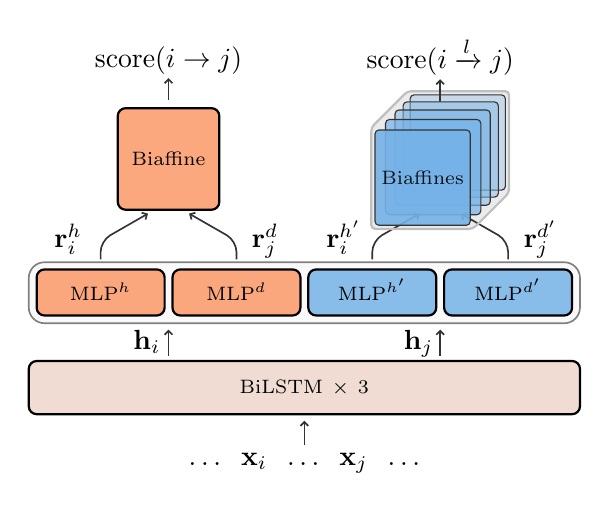
\begin{tikzpicture}[
        connect/.style={
                rounded corners=4pt,
                semithick,
                draw=black!80
            },
        arrow/.style={
                % >=latex,
                arrows = {-Straight Barb[length=0.5mm]},
                shorten >= 2pt,
                shorten <= 1.5pt,
                thin
            },
        inner arrow/.style={
                arrows = {-Straight Barb[length=0.4mm]},
                shorten >= 2pt,
                shorten <= 2pt,
                thin,
                draw=black!50
            },
        input/.style={
                rectangle,
                rounded corners=1mm,
                thin,
                dashed,
                draw=none,
                minimum width=3.5cm,
                minimum height=0.6cm,
            },
        share/.style={
                minimum height=0.5cm,
                fill={rgb,255:red,230; green,197; blue,180},
                % fill={rgb,255:red,240; green,245; blue,229},
                fill opacity=0.6,
                text opacity=1.0,
                draw=black,
                % thick,
                rounded corners=2mm,
            },
        task2/.style={
                minimum height=0.5cm,
                fill={rgb,255:red,251; green,153; blue,104},
                fill opacity=0.6,
                text opacity=1.0,
                draw=black,
                rounded corners=2mm,
            },
        label/.style={
                inner sep=0.5mm,
                fill=white,
                minimum height=0.5cm,
            },
        task1/.style={
                minimum height=0.5cm,
                fill={rgb,255:red,117; green,178; blue,231},
                draw=black,
                rounded corners=2mm
            },
        inner lstm/.style={
                fill=white,
                rectangle,
                rounded corners=1mm,
                semithick,
                % thin,
                draw=black!50,
                fill opacity=0.8
            },
        cell/.style={
                inner sep=2mm,
                rectangle,
                rounded corners=1mm,
                semithick,
                draw=black!50,
            },
        ocell/.style={
                solid,
                minimum height=0.5cm,
                rectangle,
                rounded corners=1mm,
                thick
            },
        dep arrow/.style={
        arrows = {-Latex[round,open,length=8pt,width=6pt]},
        shorten >= 2pt,
        shorten <= 1.5pt,
        thick
        }
        ]
        \centering
        \node [input, inner sep=1pt] [minimum width=4.8cm] (input) at (0, 0) {$\ldots\;\; \mathbf{x}_i \;\;\ldots\;\; \mathbf{x}_j \;\;\ldots$};
        % Concat
        \node [inner sep=0] (EmbedCat) at ($(input.north)$) {};
    
        %\scriptsize BiLSTM
        \node [share, ocell] [minimum width=7cm, minimum height=0.675cm, anchor=south] (lstm) at ($(input.north) + (0, 0.3cm)$) {\scriptsize $\mathrm{BiLSTM}\, \times \, 3$};
    

        \draw [arrow, connect] ($(EmbedCat.north) + (0cm, -0.15cm)$) -- ($(lstm.south) + (0cm, 0)$);


        % fisrt two mlps
        \node [share, fill={rgb,255:red,245; green,245; blue,245}, semithick, draw=gray] [minimum width=7cm, minimum height=0.775cm, anchor=south] (share-mlp) at ($(lstm.north) + (0cm, 0.455cm)$) {};
        

        \node [task2, ocell] [minimum width=1.625cm, minimum height=0.585cm, anchor=south west, fill opacity=0.85] (mlp-1-1-f) at ($(lstm.north west) + (0.1cm, 0.55cm)$) {};
        \node [task2, ocell] [minimum width=1.625cm, minimum height=0.585cm, anchor=south west, fill opacity=0.85] (mlp-1-1-b) at ($(lstm.north west) + (1.825cm, 0.55cm)$) {};
        \node [anchor=base] at  ($(mlp-1-1-f.south) + (0, 0.2cm)$)  {\scriptsize $\mathrm{MLP}^{h}$};
        \node [anchor=base] at  ($(mlp-1-1-b.south) + (0, 0.2cm)$)  {\scriptsize $\mathrm{MLP}^{d}$};
    
        \node [task2, ocell, fill=none, draw=none] [minimum width=1.75cm, minimum height=0.40cm, anchor=south east, fill opacity=0.5, draw opacity=0.6] (mlp-1-2-b) at ($(mlp-1-1-b.north east) + (0, 0.5cm)$) {};
    
        \node [task2, ocell, anchor=south, fill opacity=0.85, minimum height=1.29cm, minimum width=1.29cm, align=center] (arc-biaffine) at ($(mlp-1-1-f.north)!0.5!(mlp-1-1-b.north) + (0, 0.73cm)$) {\scriptsize $\mathrm{Biaffine}$};
    
        \draw [arrow, connect] ($(mlp-1-1-b.north) + (0, 0.06cm)$) -- ($(mlp-1-1-b.north) + (0, 0.35cm)$) -- ($(arc-biaffine.south) + (0.2, 0)$);
        \draw [arrow, connect] ($(mlp-1-1-f.north) + (0, 0.06cm)$) -- ($(mlp-1-1-f.north) + (0, 0.35cm)$) -- ($(arc-biaffine.south) + (-0.2, 0)$);
    
        % second two mlps
        \node [task1, ocell] [minimum width=1.625cm, minimum height=0.585cm, anchor=south east, fill opacity=0.85] (mlp-2-1-f) at ($(lstm.north east) + (-1.825cm, 0.55cm)$) {};
        \node [task1, ocell] [minimum width=1.625cm, minimum height=0.585cm, anchor=south east, fill opacity=0.85] (mlp-2-1-b) at ($(lstm.north east) + (-0.1cm, 0.55cm)$) {};
        \node [anchor=base] at  ($(mlp-2-1-f.south) + (0, 0.2cm)$)  {\scriptsize $\mathrm{MLP}^{h'}$};
        \node [anchor=base] at  ($(mlp-2-1-b.south) + (0, 0.2cm)$)  {\scriptsize $\mathrm{MLP}^{d'}$};
    
        \node [anchor=south, minimum height=1.29cm, minimum width=1.29cm, draw=none] (label-biaffine-invis) at ($(mlp-2-1-f.north)!0.5!(mlp-2-1-b.north) + (0, 0.73)$) {};
    
        \filldraw[task1, ocell, fill={rgb,255:red,235; green,235; blue,235}, draw=none, rounded corners=0.5mm] ($(mlp-2-1-f.north)!0.5!(mlp-2-1-b.north) + (-0.875, 0.5)$) -- ($(mlp-2-1-f.north)!0.5!(mlp-2-1-b.north) + (0.415, 0.5)$) -- ($(mlp-2-1-f.north)!0.5!(mlp-2-1-b.north) + (0.875, 0.96)$) -- ($(mlp-2-1-f.north)!0.5!(mlp-2-1-b.north) + (0.875, 2.25)$) -- ($(mlp-2-1-f.north)!0.5!(mlp-2-1-b.north) + (-0.415, 2.25)$) -- ($(mlp-2-1-f.north)!0.5!(mlp-2-1-b.north) + (-0.875, 1.79)$) -- cycle;
    
        \draw [arrow, connect] ($(mlp-2-1-b.north) + (0, 0.06cm)$) -- ($(mlp-2-1-b.north) + (0, 0.35cm)$) -- ($(label-biaffine-invis.south) + (0.2, 0)$);
        \draw [arrow, connect] ($(mlp-2-1-f.north) + (0, 0.06cm)$) -- ($(mlp-2-1-f.north) + (0, 0.35cm)$) -- ($(label-biaffine-invis.south) + (-0.2, 0)$);
    
        \filldraw[task1, ocell, fill=none, draw=lightgray, rounded corners=0.5mm] ($(mlp-2-1-f.north)!0.5!(mlp-2-1-b.north) + (-0.875, 0.5)$) -- ($(mlp-2-1-f.north)!0.5!(mlp-2-1-b.north) + (0.415, 0.5)$) -- ($(mlp-2-1-f.north)!0.5!(mlp-2-1-b.north) + (0.875, 0.96)$) -- ($(mlp-2-1-f.north)!0.5!(mlp-2-1-b.north) + (0.875, 2.25)$) -- ($(mlp-2-1-f.north)!0.5!(mlp-2-1-b.north) + (-0.415, 2.25)$) -- ($(mlp-2-1-f.north)!0.5!(mlp-2-1-b.north) + (-0.875, 1.79)$) -- cycle;
    
        \node [anchor=south west, minimum height=1.29cm, minimum width=1.29cm, draw=none] (label-biaffine-f) at ($(mlp-2-1-f.north)!0.5!(mlp-2-1-b.north) + (-0.875, 0.5)$) {};

        \node [anchor=north east, minimum height=1.29cm, minimum width=1.29cm, draw=none] (label-biaffine-b) at ($(mlp-2-1-f.north)!0.5!(mlp-2-1-b.north) + (0.875, 2.25)$) {};  

        \node [fill={rgb,255:red,117; green,178; blue,231}, fill opacity=0.3, minimum height=1.21cm, minimum width=1.21cm, draw=black!80, rounded corners=0.5mm, align=center, inner sep=0.1mm] at ($(label-biaffine-f)!1.0!(label-biaffine-b)$) {};
    
        \node [fill={rgb,255:red,117; green,178; blue,231}, fill opacity=0.4, minimum height=1.21cm, minimum width=1.21cm, draw=black!80, rounded corners=0.5mm, align=center, inner sep=0.1mm] at ($(label-biaffine-f)!0.8!(label-biaffine-b)$) {};
    
        \node [fill={rgb,255:red,117; green,178; blue,231}, fill opacity=0.5, minimum height=1.21cm, minimum width=1.21cm, draw=black!80, rounded corners=0.5mm, align=center, inner sep=0.1mm] at ($(label-biaffine-f)!0.57!(label-biaffine-b)$) {};

        \node [fill={rgb,255:red,117; green,178; blue,231}, fill opacity=0.7, minimum height=1.21cm, minimum width=1.21cm, draw=black!80, rounded corners=0.5mm, align=center, inner sep=0.1mm] at ($(label-biaffine-f)!0.3!(label-biaffine-b)$) {};
        
        \node [fill={rgb,255:red,117; green,178; blue,231}, fill opacity=0.9, minimum height=1.21cm, minimum width=1.21cm, draw=black!80, rounded corners=0.5mm, align=center, inner sep=0.1mm] at ($(label-biaffine-f)!0.0!(label-biaffine-b)$) {\scriptsize $\mathrm{Biaffines}$};
    
        %  LSTM -> MLP
        \draw [arrow, connect, rounded corners=1.2pt, shorten >= 2pt] ($(lstm.north) + (-1.725cm, 0)$) -- ($(share-mlp.south) + (-1.725cm, 0)$);
        \draw [arrow, connect, rounded corners=1.2pt, shorten >= 2pt] ($(lstm.north) + (1.725cm, 0)$) -- ($(share-mlp.south) + (1.725cm, 0)$);
        \node[anchor=base] at ($(share-mlp.south) + (-2cm,-0.32cm) $) {$\mathbf{h}_{i}$};
        \node[anchor=base] at ($(share-mlp.south) + (1.45cm,-0.32cm) $) {$\mathbf{h}_{j}$};
    
    
        \node[anchor=base] at ($(share-mlp.north) + (-3.0cm,0.18cm) $) {$\mathbf{r}_{i}^{h}$};
        \node[anchor=base] at ($(share-mlp.north) + (-0.5cm,0.18cm) $) {$\mathbf{r}_{j}^{d}$};
        \node[anchor=base] at ($(share-mlp.north) + (0.5cm,0.18cm) $) {$\mathbf{r}_{i}^{h'}$};
        \node[anchor=base] at ($(share-mlp.north) + (3.0cm,0.18cm) $) {$\mathbf{r}_{j}^{d'}$};
    
    
        \node[anchor=base] at ($(arc-biaffine.north) + (0cm,0.5cm) $) (arc-biaffine-label) {$\mathrm{score}(i \rightarrow j)$};
        \node[anchor=base] at ($(label-biaffine-invis.north) + (0,0.5cm) $) (label-biaffine-label) {$\mathrm{score}(i \xrightarrow{l} j)$};
    
    
        \draw [arrow, connect, rounded corners=1.2pt, shorten >= 2pt] ($(arc-biaffine-label.south) + (0, -0.25cm) $) -- ($(arc-biaffine-label.south) + (0, 0.15cm) $);
        \draw [arrow, connect, rounded corners=1.2pt, shorten >= 2pt, line cap=round] ($(label-biaffine-label.south) + (0, -0.25cm) $) -- ($(label-biaffine-label.south) + (0, 0.15cm) $);
    
    \end{tikzpicture}
    
    \caption{
      The basic architecture of Biaffine Parser. 
    }
    \label{fig:biaffine-parser}
\end{figure}
We adopt the SuPar implementation released by  \citet{zhang-etal-2020-dep}.\footnote{\url{https://github.com/yzhangcs/parser}}  
As a graph-based parser, Biaffine parser casts a tree parsing task as searching for a maximum-scoring tree from a fully-connected graph, with nodes corresponding to characters in our case. As shown in Figure \ref{fig:biaffine-parser}, it adopts standard encoder-decoder architecture, consisting of the following components.  
%Biaffine parser is a graph-based dependency parser which employs a deep biaffine scoring architecture to compute the score of each dependency and aims to find the highest-scoring dependency tree.
%\subsection{Model Architecture}
% The model architecture is shown in Figure xxx, consisting of following four components. 
% it consists of three major layers. 

\textbf{Input layer.} 
Given an input sequence, 
%consisting of $n$  $c_0c_1...c_n$, where $c_i$ is the $i$-th character and $c_0$ is a pseudo character used as tree root. 
each item is represented as a dense vector $\mathbf{x}_i$. 
For word-internal structure parsing, an item corresponds to a character, and we use char embedding. 
%the char representation output by BERT. 
%using the character embeddings $\mathbf{emb}^{c}$:
\begin{equation}
\mathbf{x}_i = \mathbf{emb}(c_i) 
% \oplus \mathbf{emb}^{bc}(c_{i-1}c_i)
\end{equation}

\textbf{BiLSTM encoder.} 
Then, a three-layer BiLSTM is applied to obtain  context-aware representations. 
We denote the hidden vector of the top-layer BiLSTM for  the i-th position as $\mathbf{h}_i$.

\textbf{Biaffine scorer.} %MLP feature abstraction.} 
Two separate MLPs are applied to each $\mathbf{h}_i$, resulting in 
%fed into two separate MLPs to 
%producing 
two lower-dimensional vectors $ \mathbf{r}_{i}^{h}$ (as head) and $\mathbf{r}_{i}^{d}$ (as dependent).
Then the score of a dependency $i \rightarrow j$ is obtained via a biaffine attention over $\mathbf{r}_{i}^{h}$ and $\mathbf{r}_{j}^{d}$. 
%To save space, we omit the 
Scoring of labeled dependencies such as $i \xrightarrow{l} j$ is analogous. 

%, representing  as a head and a dependent respectively. 
% \begin{equation}
%     \mathbf{r}_{i}^{h} = {\textup{MLP}}^{h} \left(\mathbf{h}_i \right) ;
%     \mathbf{r}_{i}^{d} = {\textup{MLP}}^{d} \left(\mathbf{h}_i \right)
% \end{equation} 
%\textbf{Biaffine classifier.} 
%The biaffine classifier computes 
% \begin{equation} \label{eq:biaffine}
%  \texttt{s}(i \leftarrow j) =  \left[
%  \begin{array}{c}
%     \mathbf{r}_{i}^{d}    \\
%       1 
%  \end{array} 
%  \right]^\mathrm{T}  \mathbf{W}^{biaffine}  \mathbf{r}_{j}^{h} 
% \end{equation} 
% where ${\mathbf{W}^{biaffine}}$ is a biaffine parameter.

% Analogously, the parser uses extra MLPs and a biaffine attention to compute scores for dependency labels. Please refer to \citet{dozat2016deep} for details.

\textbf{Decoder. }
%During decoding, the biaffine parser treats unlabeled dependency tree searching and dependency labeling as two cascaded tasks.
% First, with the scores of all dependencies, the score of a unlabeled dependency tree $\bm{y}$ is:
% \begin{equation}
% \begin{split}
% \texttt{s}(\bm{y})= \sum_{{{i \leftarrow j} \in \bm{y}}}\texttt{s}(i \leftarrow j)
% \end{split}
% \end{equation}
With the scores of all dependencies, 
we adopt the first-order algorithm of \citet{Eisner2000} % for projective decoding 
to find the optimal unlabeled dependency tree, and then independently decide the highest-scoring label for each arc. 
%$\bm{y}^{*}$ with the highest score from all the possible trees.
%Then, the biaffine parser finds the highest-scoring label for each dependency of the optimal tree $\bm{y}^{*}$.


\textbf{Training loss.} %with Local Char-wise Loss}
During training, the parser computes two independent cross-entropy losses for each position, i.e., maximizing the probability of its correct head and
%, and maximizing the probability of 
the correct label between them. 
%$c_j$ and the corresponding correct dependency label $l$ for each character $c_i$ independently.
% \begin{equation}
% \begin{split}
%  \texttt{loss}(i \xleftarrow{l} j) = &-\log{ 
% \frac{e^{\texttt{s}(i \leftarrow j)}}
% {\sum\limits_{0 \le k \le n, k \neq i}e^{\texttt{s}(i \leftarrow k)}} 
% }\\
% & -\log{ 
% \frac{e^{\texttt{s}(i \xleftarrow{l} j)}}
% {\sum\limits_{l' \in \mathcal{L}}e^{\texttt{s}(i \xleftarrow{l'} k)}} 
% }
% \end{split}
% \end{equation}
% where $\texttt{s}(i \xleftarrow{l} j)$ is the score of labeling the dependency $i \leftarrow j$ as $l$. $\mathcal{L}$ is the whole dependency label set.





%\subsection{Experiments and results}
\subsection{Settings}

\textbf{Data.} We randomly split all words in WIST into three parts, 2,500/5,000 as development/test data and remaining as training data. 
%We conduct experiments on our manually annotated char-level syntactic treebank, which consists of 25,531, 2,504, and 5,013 words in training, development, and test sets respectively.

\textbf{Hyperparameters.} 
We set the dimension of char embeddings to 100. 
We obtain pre-trained character embeddings by training  word2vec on Chinese Gigaword Third Edition.
%We adopt the 100 dimension character embeddings of %\citet{liying-2019} 
%pretrained with word2vec model on Chinese Gigaword.
In order to see effect of contextualized character representations, we apply BERT \cite{devlin-2019-bert} \footnote{BERT-base-Chinese:\url{https://github.com/google-research/bert}} to each word as a char sequence. The output vectors of the top four layers are concatenated and reduced into a dimension of 100 via an MLP. 
For other hyper-parameters, we keep the default configuration in SuPar.
%We adopt most of the parameter settings in the open source parser \cite{dozat2016deep}. 
%Each model is trained for at most 1000 iterations. We stop training when the peak performance on the development data does not increase in 100 consecutive iterations. 


%The dimension of char embedding is set to 50. 
\textbf{Evaluation metrics.} 
We adopt the standard unlabeled and labeled attachment score (UAS/LAS), i.e., the percent of characters that receives the correct head (and label). 
%The unlabeled and labeled complete matches (UCM/LCM) is the percent of words having correct whole trees.
The complete match (CM) is the percent of words having correct whole trees.

\setlength{\tabcolsep}{3.6pt}
\begin{table}[tb]
%\setlength{\leftskip}{-25pt}
\begin{center}
% \begin{small}
\begin{tabular}{l  rr rrr }
\toprule
\multirow{2}{*}{} 
& \multicolumn{2}{c}{Dev }
& \multicolumn{3}{c}{Test} \\
\cmidrule(lr){2-3} \cmidrule(lr){4-6}
% \cline{2-6}
& UAS & LAS & UAS & LAS & CM\\
\hline
Random & 81.18 & 76.15  & 80.63 & 75.58 & 65.13 \\[2pt]
%\hline
\multirow{2}*{Pretrained}
 & 82.42 & 77.30 & 81.64 & 76.98  & 67.09 \\
 & +1.24 & +1.15 & +1.01 & +1.40 & +1.96\\[2pt]
%\hline
\multirow{2}*{BERT} 
 & 88.27 & 85.18 & 88.33 & 84.98 &77.72\\
 & +5.85 & +7.88 & +6.69 & +8.00 & +10.63\\
\bottomrule
\end{tabular}
% \end{small}
\caption{Results of word-internal structure parsing using different character representations.} 
\label{iwdp-result}
\end{center}
\end{table}


\subsection{Results}

Table \ref{iwdp-result} shows the main results  %word-internal structure parsing 
under different char representations.  
% It turns out that word-internal structure parsing is not a piece of cake.
% The best model integrated BERT representations\footnote{The BERT in the experiment is ``bert-base-chinese'' released by \citet{peters2018deep}.}, which outperforms those without BERT  by over 10 in LAS, merely achieves a LAS of 84.98 and a LCM of 77.72.
% Pretrained char embeddings are also helpful to the word-internal structure parsing.
% But it only brings improvement by 1.40 in LAS and 1.96 in LCM, compared with the model using randomly initialized char embeddings.
It is obvious that using randomly initialized char embeddings, the parser can only reach about 76 in LAS. This shows that parsing word-internal structure is very challenging without using extra resources. 
When we pretrain char embeddings on large-scale labeled data, the performance can be consistently improved by over 1 point in both UAS/LAS, and nearly 2 points in CM. 
Finally, employing the contextualized character representations dramatically improves performance further by about 6/8/10 points in UAS/LAS/CM. 

However, even with BERT, model performance still lags behind averaged human performance (90.9 in LAS) by large margin.
Our experienced annotators can even reach more than 94. 
Our experience in manual annotation points out two possible directions to enhance the model: 1) making use of sentence-level contextual information; 2) leveraging the meanings in dictionaries, usually in the form of explanation or example sentences. 
We leave them for future exploration. 

%without  using pretrained char embeddings brings substantial improvement by 1.40 in LAS and 1.96 in LCM on test. 

%Integrating with BERT representations\footnote{The BERT in the experiment is ``bert-base-chinese'' released by \citet{peters2018deep}.} can further boost the model performance by a very large margin, outperforming those without BERT by over 8 in LAS and over 10 in LCM on test. 

\textbf{Analysis on label-wise accuracy.}
% Using BERT representations can further improve the parser by a very large margin.
%\begin{figure}[tb]
  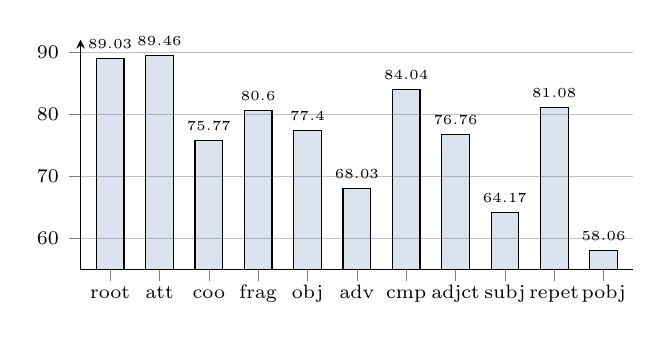
\begin{tikzpicture}
    \begin{axis} [
        width=8.6cm, height=4.5cm,
        ybar,
        axis y line=left,
        axis x line=left,
        x axis line style={-},
        ymajorgrids=true,
        enlarge x limits=0.06,
        tick align=outside,
        ymin=55, ymax=92,
        symbolic x coords={
            root, att, coo, frag, obj, adv, cmp, adjct, subj, repet, pobj
        },
        xtick=data,
        nodes near coords=\pgfmathprintnumber\pgfplotspointmeta,
        xticklabel shift=6,
        x tick label style={anchor=base, font=\scriptsize},
        y tick label style={font=\scriptsize},
    ]
    \addplot [
        draw=black,
        fill opacity=0.2, 
        text opacity=1,
        font=\tiny, 
        fill={rgb,255:red,76; green,114; blue,176}] coordinates {
        (root, 89.03)
        (att, 89.46)
        (coo, 75.77)
        (frag, 80.6)
        (obj, 77.4)
        (adv, 68.03)
        (cmp, 84.04)
        (adjct, 76.76)
        (subj, 64.17)
        (repet, 81.08)
        (pobj, 58.06)
    };
  \end{axis}
\end{tikzpicture}

\caption{
  Accuracy on different dependency labels.
}
\label{fig:model-acc}
\end{figure}

The second major row in Table \ref{table:label distribution} reports accuracy regarding different labels for the model with BERT. 
The model achieves the highest accuracy on ``att'' and ``root'', possibly because the two labels take very large proportion in the data for sufficient model training. 
%One direct reason is that these two labels accounts for the largest proportion of all labels, and thus the model can be trained sufficiently. 
% , indicating that it is relatively easy for the model to recognize the head character for each word.
%Moreover, it is easy to recognize ``att'' since the word with ``att'' label usually has a typical modifier-noun structure, which is very common in Chinese words and usually frequently occurs in the training data. 
%For ``root'', it represents the most important head character that conveys the main meaning of each word, such head characters are also high-frequency characters and thus can be distinguished with other unimportant characters. 
By contrast, ``pobj'' and ``subj'' have the lowest accuracy, and are difficult for models as well as discussed in Section \ref{sec:data-annotation}. 
%performance, achieving only ``58.1'' in accuracy.
%By carefully checking the predicted results, we find that the model usually confuses ``pobj'' with ``obj''. In fact, these two labels are quite similar in syntax. The proportion of ``obj'' is much larger than ``pobj'' (5.4 vs. 0.2). The sample imbalance problem causes the model to lean to label ``pobj'' as ``obj''.
This leads to 
another observation that model accuracy is roughly correlated with annotation accuracy, implying the difficulties for human and model are usually consistent. 
% However, it is not easy for the model to correctly recognize ``subj'' and ``pobj'', achieving only ``64.2'' and ``58.1'' in accuracy respectively. By carefully checking the predicted results, we find that the model usually confuses ``subj'' with  ``adv'' and confuses ``obj'' with ``pobj''.

% the sample imbalance problem causes the model to lean to label “激动(excite)” as an adjective



% as illustrated in Table \ref{table:label distribution}, and thus the model can be trained sufficiently. 

% coo和adv容易混淆

% and ``att''

% the proportion of these 

% account for a relatively large proportion in all the labels


% whereas the lowest accuracy on ``subj'' and ``pobj'', which is consistent with the manual annotation accuracy.



% root和att准确率高是因为:1.root标签属于核心字,是一个词中最为核心的部分,往往承载着一个词的主要意思,因此比较容易找出。att标签准确率高我觉得是因为att标签数量多,如果核心字是名词性字,那么它前面的字很有可能是att,容易识别,特征明显。subj难识别是因为,subj标签容易被误标注成adv标签,对于是主语还是修饰关系,有时候难以理解,pobj标签错误率高更大原因是因为难以分辨到底是obj还是pobj,比如在这个字,一般认知下会觉得是介词,但是其实在单个字中,在通常作为动词,形成obj



%\input{content/encode-iwdp-for-dependency}
% \section{Sentence-level syntactic Parsing with Structure-aware Word Representation}

\section{Utilizing Word-internal Structure}

This section presents a preliminary study on utilizing word-internal structure, aiming to address the third question: is modeling word-internal structures beneficial for word representation learning? 
% We conduct our study on sentence-level dependency parsing to make investigation on whether integrating structure-aware word representation can be beneficial. 
% 【用解释为啥在句法分析上做实验吗?】

We use sentence-level dependency parsing as the focusing task \cite{KublerDEP09}, mainly considering resemblance in tree structure representation and close relatedness between the two tasks. 
% We also 
Given an input sentence $w_0w_1...w_m$, 
%where $w_i$ is  the $i$-th word and $w_0$ is a pseudo word for sentence start, sentence-level dependency 
the goal of dependency parsing is to find an optimal dependency tree for the sentence. 
%the head word $w_j$ for each word $w_i$ and the dependency relation label between $w_i$ and $w_j$.
%Similar to the word-internal structure parsing as described in Section \ref{char-pasrsing}, w
Again, we adopt SuPar \cite{zhang-etal-2020-dep} for implementation of Biaffine parser \cite{dozat2016deep} % and the implementation of  
as our basic parser. 
%for sentence-level dependency parsing. 


\subsection{Methods}

The basic parser applys a BiLSTM over character sequence to obtain word representation. 
In this part, we propose two  simple alternative methods to encode internal structure shown in Figure \ref{fig:example}-(c).

\textbf{Basic CharLSTM method.} For each word, the basic Biaffine parser uses the concatenation of word embeddings and CharLSTM outputs to represent each word in the input layer:
\begin{equation}\label{eq:charlstm-eq}
\begin{split}
& \mathbf{x}_i = \mathbf{emb}(w_i) 
 \oplus \textup{CharLSTM}(w_i) \\
& \textup{CharLSTM}(w_i) \leftarrow \textup{BiLSTM}(...,\mathbf{z}_{k},...) \\
& \mathbf{z}_{k} = \mathbf{emb}(c_{i,k}) 
\end{split}
\end{equation}
where $c_{i,k}$ is the k-th character of $w_i$. The final word representation from $\textup{CharLSTM}(w_i)$ 
is obtained by concatenating two last-timestamp hidden output vectors of a one-layer BiLSTM. 
%The other parts of the model architecture for the sentence-level dependency parsing remain consistent with the word-internal structure parsing as described in section \ref{char-pasrsing}.

% To exploit the syntactic word-internal information for sentence-level parsing, we investigate and compare two methods to encode the syntactic word-internal structures.
% Each method produces a representation considering the word-internal structure of the concerned word $w_i$, which is denoted as $\mathbf{r}_i^{syn}$.
% We treat the syntactic structure-aware representation $\mathbf{r}_i^{syn}$ of word $w_i$ as extra features and concatenate it with the original input $\mathbf{x}_i^w$.
% We introduce the two methods in detail in the following subsections.


\textbf{LabelCharLSTM Method.} 
% 谁的方法说明,用label embedding就很有效果了。
% \textbf{Encoding with sequence model.}
%Previous work on syntax-aware semantic role labeling shows it is simple and effective to %of using syntactic trees is to 
%feed syntactic label embeddings as extra inputs into encoders \cite{XXXX}. 
Considering that the word is usually very short and a bare label itself provides rich syntax information,  
we propose a straightforward extension to CharLSTM, named as LabelCharLSTM, via minor modification.%  to Equation \ref{eq:charlstm-eq}.
\begin{equation}\label{eq:labelcharlstm-eq}
\begin{split}
& \mathbf{z}_{k} = \mathbf{emb}(c_{i,k}) \oplus \mathbf{emb}(l_{i,k})
\end{split}
\end{equation}
where $l_{i,k}$ represents the label between $c_{i,k}$ and its head in the word-internal structure. 
%concatenating char with label embedding 
% Apart from the novel graph neural network, we also utilize CharLSTM, without changing the major network structure of baseline model, to integrate structure-aware word representations.
% 除了使用新颖的图神经网络之外,我们还给出另外一个十分直接的引入字结构表示信息的方法,which 我们不需要引入别的神经网络结构。
% 师姐我说我们用charLSTM编码label的初衷是,
% In syntactic parsing task, one of the most important role of the CharLSTM is to explore the part-of-speech clues of a word from characters it contained.
% For Chinese language, 【可以说,中心词以及非中心字的语法角色隐含了词性信息吗? 比如``枣红''的中心字是``红'',而``红枣''的中心字是``枣''】.
%As depicted in Table \ref{table:summary-different-num-word}, about $92.1\%$ words in the dataset are one-character words or two-character words.
%Their word-internal skeleton trees are simple, but the word-internal dependency labels still can provide clues. We encode such dependency label information by employing a BiLSTM.
% by pointing out center-character and illustrating the function of non-center-characters.
% So, we omit the arcs of the word-internal structures.
% , and feed each character together with its relation labels into the CharLSTM.
% That is, for now, the input of CharLSTM in Equation \ref{baseline-input} is $w_i$ and $l_{u,v}$, the label of dependency $u \leftarrow v$. 【这里的的公式还有些奇怪,得再改一下】
% 在依存解析中,charLSTM的一个很重要的任务是去从组成词的字中发掘POS信息。我们发现基于这个出发点 词内部的每个字的label要比字符间的依存弧更为重要,因为它可以指出哪个字为词语的中心字并标明不同字在词语中所承担的角色。因此我们为了使得模型更加简单而忽略arc。
%Formally, we concatenate the character embedding with the dependency label embedding, and then go through a single-layer BiLSTM:
% \begin{equation}
%     % [\overrightarrow{\mathbf{h}}_{u}, \overleftarrow{\mathbf{h}}_{u} ] =\textup{BiLSTM}(\mathbf{emb}^{c}(c_u) \oplus \mathbf{emb}^{l}(l_{u,v}))
%     {\mathbf{h}}_{u} =\textup{BiLSTM}(\mathbf{emb}^{c}(c_u) \oplus \mathbf{emb}^{l}(l_{u,v}))
% \end{equation}
% Here, $\mathbf{emb}^{l}(l_{u,v})$ is the label embedding for dependency $u \leftarrow v$.
% The pooling operation is performed on the top-layer ouputs of BiLSTM to obtain $\mathbf{r}_i^{syn}$, which is the same as Equation \ref{pooling}. 



% \subsection{Representation with GCN}
% We employ two different models to encode syntactic word-internal structures explicitly.
\textbf{LabelGCN method.} 
%缩写应该在intro提到才对,到时候确认
% \textbf{Encoding with graph model.} 
Previous work show that GCN is very effective in encoding
%The graph convolutional network (GCN) \cite{kipf2016semi} is designed for modeling graph structures, and can be naturally used for exploiting
syntactic trees \cite{marcheggiani-titov-2017,zhang-etal-2018}. 
%In this work, we employ GCN to encode the word-internal structure of Chinese words. 
We follow the implementation of \citet{zhang-etal-2018} and use a two-layer GCN as a more sophisticated way. % to encode word-internal structure. 
In order to utilize labels, we extend vanilla GCN to have the same input with 
% Formally, given a internal structure of a word with $t$ nodes (each node is a character), we use an $t \times t$ adjacency matrix $\mathbf{{A}}$ to represent such structure, where $A_{uv}=1$ if there is a dependency arc between the $u$-th node $c_u$ and the $v$-th node $c_v$. Following \citet{marcheggiani-titov-2017}, we also set the diagonal elements of $\mathbf{{A}}$ to $1$ to add a self-loop for each node.
% The input of GCN is the same with
LabelCharLSTM, i.e., $\mathbf{z}_{k}$.
We obtain the final word representation by performing average pooling over the output vectors of the top-layer GCN.  
% The representation vector $\mathbf{h}_u^m$ of the node $c_u$ at the $m$-th layer of GCN is computed based on its one-hop neighbours and itself, which is defined as:
% \begin{equation}\label{GCN}
%     \begin{split}
%     \mathbf{h}_{u}^{m}&=\rho\Bigg( \sum_{v=1}^{n}{\mathbf{{A}}_{uv}}\mathbf{W}^{m}\mathbf{h}_v^{m-1} + \mathbf{b}^{m}\Bigg)
%     \end{split}
% \end{equation}
% where $\mathbf{W}^{m}$ and $\mathbf{b}^{m}$ are model parameters. $\rho$ denotes an activation function. 
% $\mathbf{h}_u^0$ is the initial input representation to GCN, which is the concatenation of the character embedding and the dependency label embedding.
% \begin{equation}
%     \mathbf{h}_{u}^{0}=\textup{BiLSTM}(\mathbf{emb}^{c}(c_u) \oplus \mathbf{emb}^{l}(l_{u,v}))
% \end{equation}
% Here, $\mathbf{emb}^{l}(l_{u,v})$ is the label embedding for dependency $u \leftarrow v$.
% 【h0不用BiLSTM了,后面改】
% 【双向还没写,看实验结果】
% The final syntactic structure-aware representation $\mathbf{r}_i^{syn}$ for the word $w_i$ is obtained by performing an average pooling operation on the top-layer outputs of the GCN which contains $M$ layers in total.
% % Finally, an average pooling operation is performed on the top-layer GCN outputs to obtain the syntactic structure-aware representation $\mathbf{r}_i^{syn}$ for the word $w_i$.
% \begin{equation}
% \mathbf{r}^{syn}_{i} =
% \textup{Pooling}(\{\mathbf{h}_u^M|1 \leq u \leq t\})
% \label{pooling}
% \end{equation}

%\subsection{Representation with BiLSTM}
% \textbf{Encoding with sequence model.}
Apart from the novel graph neural network, we also utilize CharLSTM, without changing the major network structure of baseline model, to integrate structure-aware word representations.
% 除了使用新颖的图神经网络之外,我们还给出另外一个十分直接的引入字结构表示信息的方法,which 我们不需要引入别的神经网络结构。
% 师姐我说我们用charLSTM编码label的初衷是,
% In syntactic parsing task, one of the most important role of the CharLSTM is to explore the part-of-speech clues of a word from characters it contained.
% For Chinese language, 【可以说,中心词以及非中心字的语法角色隐含了词性信息吗? 比如``枣红''的中心字是``红'',而``红枣''的中心字是``枣''】.
As depicted in Table \ref{table:summary-different-num-word}, about $92.1\%$ words in the dataset are one-character words or two-character words.
Their word-internal skeleton trees are simple, but the word-internal dependency labels still can provide clues. We encode such dependency label information by employing a BiLSTM.
% by pointing out center-character and illustrating the function of non-center-characters.
% So, we omit the arcs of the word-internal structures.
% , and feed each character together with its relation labels into the CharLSTM.
% That is, for now, the input of CharLSTM in Equation \ref{baseline-input} is $w_i$ and $l_{u,v}$, the label of dependency $u \leftarrow v$. 【这里的的公式还有些奇怪,得再改一下】
% 在依存解析中,charLSTM的一个很重要的任务是去从组成词的字中发掘POS信息。我们发现基于这个出发点 词内部的每个字的label要比字符间的依存弧更为重要,因为它可以指出哪个字为词语的中心字并标明不同字在词语中所承担的角色。因此我们为了使得模型更加简单而忽略arc。
Formally, we concatenate the character embedding with the dependency label embedding, and then go through a single-layer BiLSTM:
\begin{equation}
    % [\overrightarrow{\mathbf{h}}_{u}, \overleftarrow{\mathbf{h}}_{u} ] =\textup{BiLSTM}(\mathbf{emb}^{c}(c_u) \oplus \mathbf{emb}^{l}(l_{u,v}))
    {\mathbf{h}}_{u} =\textup{BiLSTM}(\mathbf{emb}^{c}(c_u) \oplus \mathbf{emb}^{l}(l_{u,v}))
\end{equation}
Here, $\mathbf{emb}^{l}(l_{u,v})$ is the label embedding for dependency $u \leftarrow v$.
The pooling operation is performed on the top-layer ouputs of BiLSTM to obtain $\mathbf{r}_i^{syn}$, which is the same as Equation \ref{pooling}. 
% The final syntactic structure-aware representation $\mathbf{r}_i^{syn}$ 
% The final representation $\mathbf{r}_i^{syn}$ is the concatenation of $\overrightarrow{\mathbf{h}}_{n}$, the forward hidden representation of the last word of the sentence, and $\overleftarrow{\mathbf{h}}_{0}$, the backward representation of the first word.
% The final representation $\mathbf{r}_i^{syn}$ is the top-layer BiLSTM outputs.





% In addition to directly encoding the syntactic word-internal tree structure with the graph model GCN, we also employ the sequence model BiLSTM to obtain the structure-aware word representation.

%\input{content/encode-iwdp-exp}


%\subsection{Experiments and results}
\subsection{Experiments}

\paragraph{Settings.} Following \citet{chen-manning-2014fast}, we conduct experiments on CTB5 with the same data split (16,091/803/1,910 sentences) and constituent-to-dependency conversion. 
%(CTB5) with dependencies obtained by the Penn2Malt tool \footnote{http://stp.lingfil.uu.se/∼nivre/research/Penn2Malt.html}. 
%Most of the hyper-parameter settings is adopted from \citet{dozat2016deep}, expect settings of CharLSTM.
Both char/label embeddings are randomly initialized and have the same dimension of 50. 
For the parsers using gold-standard POS tags, we randomly initialized the POS tagging embeddings and set the dimension to 50.
For other hyperparameters, we adopt the default configuration of SuPar, including the pre-trained word embeddings. 
%We adopt the de
%and hidden layer of CharSLTM are set to 50. 
% We also obtain pre-trained word embeddings by training word2vec on Chinese Gigaword V3.
%Third Edition 【todo 是否用缩写?】

For multi-char words without annotated internal structure, we use the automatic outputs from the trained parser with BERT in Section \ref{sec:WIS-parsing}, so that every word corresponds to a single structure.  
%实验部分要给出所有词的词内部结构怎么来的。预测。
%所有词的内部结构都是给定的,每个词给一个。

We use word-wise UAS/LAS/CM for evaluation, and punctuation is excluded in all metrics.
% We adopt the same data split as \citet{zhang-clark-2008} on CTB5 and the gold standard data split on CoNLL09.
% Then, we obtain dependencies from CTB5 by the Penn2Malt tool \footnote{http://stp.lingfil.uu.se/∼nivre/research/Penn2Malt.html} and find corresponding constituent trees from Chinese Penn Treebank 6.0 (CTB6) according to CoNLL09 data.
% For dependency parsing, we use unlabeled and labeled attachment score (UAS/LAS) as main metrics. 
% For constituent parsing, we use the standard constituent-level labeled precision, recall and F-score (P/R/F) as the evaluation metric.

\paragraph{Main results.}

Table \ref{table:results-dependency} shows the parsing performance. We can see that both LabelCharLSTM and LabelGCN substantially outperform the basic CharLSTM method. 
LabelGCN achieves the best performance on UAS and LAS, with a gain of 0.71 and 0.80 respectively. 

The fourth row reports performance of LabelGCN without using label embedding, leading to consistent accuracy drop, demonstrating the usefulness of rich labels, which is a key contribution of this work, despite the extra annotation effort. 
%Without encoding word-internal skeleton tree, the BiLSTM approach already achieves improvement of 0.37/0.47 in UAS/LAS.
%Integrating the arc information by using GCN can further improve parsing performance by 0.56/0.63 in UAS/LAS.

% \begin{table}[tb]
% \setlength{\tabcolsep}{6.5pt}
% \centering
% \begin{tabular}{lccccc}
%     \toprule
%     & \multicolumn{2}{c}{Dev} & \multicolumn{3}{c}{Test} \\
%     & UAS & LAS & UAS & LAS & CM \\[2pt]
%     \hline
%     \\[-8pt]
%     Baseline &87.03 &85.05 &87.31 &85.23 &30.73 \\
%     BiLSTM   &87.03 &\textbf{85.22} &87.68 &85.70 &31.68 \\
%     GCN      &\textbf{87.13} &85.19 &\textbf{87.87}  &\textbf{85.86} & \textbf{31.78} \\
%     GCN w/o label &86.87 &84.76 &87.55 &85.41 &31.36\\
%     GCN 波浪 &87.06 &85.05 &87.56 &85.47& 31.15  \\

%     \bottomrule
% \end{tabular}
%     \caption{Main results for dependency parsing.}
%     \label{table:results-dependency}
% \end{table}

% \begin{table}[tb]
% \setlength{\tabcolsep}{6.5pt}
% \centering
% \begin{tabular}{lccccc}
%     \toprule
% %    &  \multicolumn{3}{c}{Test} \\
%     &  UAS & LAS & CM \\
%     \hline
%     Basic CharLSTM &87.31 &85.23 &30.73 \\
%     LabelCharLSTM    &87.68 &85.70 &31.68 \\
%     \hline
%     LabelGCN       &\textbf{87.87}  &\textbf{85.86} & \textbf{31.78} \\
%     %\hline
%     $~~~~~$ w/o label  &87.55 &85.41 &31.36\\
% %    $~~~~~$ GCN 波浪  &87.56 &85.47& 31.15  \\
%     \bottomrule
% \end{tabular}
%     \caption{Parsing performance on CTB5-test.}
%     \label{table:results-dependency}
% \end{table}

\begin{table}[tb]
\setlength{\tabcolsep}{6.5pt}
\centering
\begin{tabular}{lccccc}
    \toprule
%    &  \multicolumn{3}{c}{Test} \\
    &  UAS & LAS & CM \\
    \hline
    Basic CharLSTM &88.31 &85.96 &32.04 \\
    LabelCharLSTM    &88.78 &86.51 &\textbf{33.19} \\
    \hline
    LabelGCN       &\textbf{89.02}  &\textbf{86.76} & 32.93 \\
    %\hline
    $~~~~~$ w/o label  &88.66 &86.28 &32.20\\
%    $~~~~~$ GCN 波浪  &87.56 &85.47& 31.15  \\
    \bottomrule
\end{tabular}
    \caption{Parsing performance on CTB5-test.}
    \label{table:results-dependency}
\end{table}

%\input{content/encode-iwdp-analysis}

% \begin{table}[tb]
% \setlength{\tabcolsep}{2pt}
% \centering
% \begin{tabular}{lcccccc}
%     \toprule
%     % \hline
%     & \multicolumn{3}{c}{Dev} & \multicolumn{3}{c}{Test} \\
%     & P & R & F & P & R & F \\[2pt]
%     \hline
%     \\[-8pt]
%     \multicolumn{7}{c}{CTB5} \\
%     Baseline &87.81 &86.36 &87.08 &87.42 &87.13 &87.27 \\
%     BiLSTM   &\textbf{88.12} &\textbf{86.82} &\textbf{87.46} &\textbf{87.80} &\textbf{87.45} &\textbf{87.62} \\
%     GCN      &87.73 &86.56 &87.14 &87.60 &87.33 &87.47\\
%     \hline
%     \\[-8pt]
%     \multicolumn{7}{c}{CoNLL09} \\
%     Baseline &88.35 &87.35 &87.84 &88.66 &87.58 &88.12 \\
%     BiLSTM &88.69 &87.76 &88.22 &88.85 &87.84 &88.34 \\
%     GCN & \\[2pt]

%     \bottomrule
% \end{tabular}
%     \caption{Main results for constituency parsing.}
%     \label{table:results-constituency}
% \end{table}


\begin{table}[!tb]
\setlength{\tabcolsep}{4.2pt}
\centering
\begin{tabular}{lrrrr}
    \toprule
    % \hline
   & all & $>2$ &$\le2$ & unk.  \\
    \hline
    % \\[-8pt]
    Basic CharLSTM &85.96& 86.42 &82.03 &81.73   \\[2pt]
    \multirow{2}*{LabelGCN} 
    &86.76& 87.10 &83.79 &84.30  \\
    & +0.80 &+0.68 & +1.76 &+2.57  \\
    \bottomrule
\end{tabular}
    \caption{Parsing LAS regarding to word frequency.}% of common/rare/unkown words.} % frequency}. % on CTB5-test.}
    \label{table:rare-word-las}
\end{table}

\paragraph{Analysis on rare words.} 
To gain more insights on how word-internal structure helps word representation learning, we divide the words in CTB5-test into several groups according to their frequency in CTB5-train, and report fine-grained accuracy in Table \ref{table:rare-word-las}. 
%To investigate whether our proposed word-internal structure can be beneficial to the parsing performance on rare words, we divide the words on test data into three categories according to their frequency on training data: words with frequency $\leq 2$, words with frequency $\leq 1$ and words out of the training data (OOV). Table \ref{table:rare-word-las} compares the parsing performance (LAS) of the baseline model and our model which encodes word-internal structure with GCN on the three categories. We also give the performance on the whole test data (overall) for reference. We observe that the improvements on the rare words and OOV words are consistently larger than that on the whole test data, which means the word-internal structures make more contribution to rare/OOV words than high-frequency words. The main reason is that the word-internal structures contain rich information on how multiple characters form a word, which is helpful for representing rare words via composing the meanings of characters.
We can see that the overall performance gain is mostly contributed by improvement over rare words with low frequency or totally unknown. 
This verifies that word-internal structures can help the model to better represent rare words. 


\begin{table}[t]
\setlength{\tabcolsep}{2.5pt}
\centering
\begin{tabular}{lrrrrr}
    \toprule
%    &  \multicolumn{3}{c}{Test} \\
    &  UAS & LAS \\
    \hline
    % \citet{chen-manning-2014fast} & 88.1 &85.7\\
%   \citet{ballesteros-2016-training}& 87.65&86.21&\\
%   \citet{kiperwasser-2016-simple} &87.6 &86.1&\\
%   \citet{acl16-Zhang-parsing} & 87.65 & 86.17 &\\
%   \citet{kuncoro-2016-distilling} &88.87 &87.30 \\
   \citet{ma-2017-neural} &89.05 &87.74 \\
   \citet{dozat2016deep} &89.30 &88.23 \\
%   Zheng (2017) & 89.42 &87.94\\
%   \citet{coling2018-seq2seqparsing} &88.78 &86.23\\
   \citet{acl18-ma-stackpointer} &\textbf{90.59}&\textbf{89.29}\\
    \hline
    Basic CharLSTM &91.11 &89.91  \\
    LabelCharLSTM    &\textbf{91.31} &90.15 \\
    LabelGCN       &\textbf{91.31}  &\textbf{90.16} \\
    %\hline
    % $~~~~~$ w/o label  &87.55 &85.41 &31.36\\
%    $~~~~~$ GCN 波浪  &87.56 &85.47& 31.15  \\
    \bottomrule
\end{tabular}
    \caption{Parsing performance with gold-standard POS tags on CTB5-test.}
    \label{table:results-dependency-goldpos}
\end{table}


\paragraph{Results with gold-standard POS tags.} As suggested by a reviewer, we train our parser with gold-standard POS tags by concatenating the original input (i.e., $\mathbf{x}_{i}$ in Equation \ref{eq:charlstm-eq}) with gold-standard POS tag embeddings, in order to compare with previous works. 
Table \ref{table:results-dependency-goldpos} shows the results. 
Compared with the Basic CharLSTM results in Table \ref{table:results-dependency}, using gold-standard POS tags as extra features for the Basic CharLSTM leads to substantial improvements by 2.80 and 3.95 in UAS and LAS respectively, and outperforms the previous works as presented in Table \ref{table:results-dependency-goldpos}, showing that the basic CharLSTM can be served as a strong baseline model.


% the Basic CharLSTM, LabelCharLSTM, and LabelGCN in Table \ref{table:results-dependency-goldpos} augment the input by concatenating the original input (i.e., $\mathbf{z}_{k}$) with the embeddings of gold-standard POS tags.

% When using gold-standard POS tags as extra features, the basic CharLSTM outperforms the previous works, showing that the basic CharLSTM can be served as a strong baseline model.

Compared with the Basic CharLSTM, utilizing word-internal structure with LabelCharLSTM or LabelGCN achieves consistently better performance by 0.24 and 0.25 respectively in LAS in the scenario of using gold-standard POS tags.
Besides the strong baseline, another reason that the improvement brings by the internal-word structure is slight when using gold-standard POS tags is that a part of linguistic information in the POS tags and the word-internal structures may be overlapping.

% less than that in the scenario of without using gold-standard POS tags


% Although the improvement is less than that in the scenario of without using gold-standard POS tags due to a part of overlapping information in POS tags and internal-word structures, we believe that the POS tags and internal-word structures can also provide complementary contributions to the parsing performance according to the slightly but consistently improvement. 
% We will explore





% \subsection{Unsupervised Grammar Induction}

\subsubsection{Setup}\label{sec:LM_setup}
\paragraph{Baselines and Evaluation.} 
For comparison, we include six recent strong models for unsupervised parsing with available open source implementations: StructFormer \cite{DBLP:conf/acl/ShenTZBMC20}, Ordered Neurons~\cite{DBLP:conf/iclr/ShenTSC19}, URNNG~\cite{dblp:conf/naacl/kimrykdm19}, DIORA~\cite{dblp:conf/naacl/drozdovvyim19}, C-PCFG~\cite{kim-etal-2019-compound}, and R2D2~\cite{hu-etal-2021-r2d2}. 
To observe the marginal gain from pretraining, we also include Fast-R2D2 without pretraining denoted as Fast-R2D2$_{\rm w/o}$.
Following~\newcite{htut-etal-2018-grammar}, we train all systems on a training set consisting only of raw text, and evaluate and report the results on an annotated test set. 
As an evaluation metric, we adopt sentence-level unlabeled $F_1$ computed using the script from \newcite{kim-etal-2019-compound}.
We compare against the non-binarized gold trees per convention.
The results of Fast-R2D2 are obtained from 3 runs of each model with different random seeds in pre-training.
The best checkpoint for each system is picked based on scores on the validation set. 
Fast-R2D2 is pretrained with span constraints for the word level but without span constraints for the word-piece level.
To support word-piece level evaluation, 
we convert gold trees to word-piece level trees 
by simply breaking each terminal node into a non-terminal node with its word-pieces as terminals, e.g., (NN discrepancy) into (NN (WP disc) (WP \#\#re) (WP \#\#pan) (WP \#\#cy)).

\paragraph{Environment.} EFLOPS~\cite{DBLP:conf/hpca/DongCZYWFZLSPGJ20} is a highly scalable distributed training system designed by Alibaba. With its optimized hardware architecture and co-designed supporting software tools, including ACCL~\cite{DBLP:journals/micro/DongWFCPTLLRGGL21} and KSpeed (the high-speed data-loading service), it could easily be extended to 10K nodes (GPUs) with linear scalability.

\paragraph{Hyperparameters.} The tree encoder of our model uses 4-layer Transformers with 768-dimensional embeddings, 
3,072-dimensional hidden layer representations, and 12 attention heads. 
The top-down parser of our model uses a 4-layer bidirectional LSTM with 128-dimensional embeddings and 256-dimensional hidden layer. The sampling number $K$ is set to be 256.
Training is conducted using Adam optimization with weight decay using a learning rate of $5 \times 10^{-5}$ for the tree encoder and $1 \times 10^{-2}$ for the top-down parser.
The batch size is set to 64 per GPU for $m$=$4$, though we also limit the maximum total length for each batch, such that excess sentences are moved to the next batch. The limit is set to 1,536. It takes about 120 hours for 60 epochs of training with $m$=$4$ on 8 A100 GPUs.

\paragraph{Data.}  For English, to fully leverage the scalability of Fast-R2D2, we pretrain Fast-R2D2 on WikiText103~\cite{DBLP:conf/iclr/MerityX0S17}
and then fine-tune the model on the Penn Treebank (PTB)~\cite{marcus-etal-1993-building}
for 10 epochs with the same objective.
WikiText103 is split at the sentence level, and sentences longer than 200 after tokenization are discarded (about 0.04‰ of the original data). 
The total number of sentences is 4,089,500, and the average sentence length is 26.97.
For Chinese, we use a subset of Chinese Wikipedia (Simplified Characters) for pretraining, specifically the first 10,000,000 sentences shorter than 150 characters and then fine-tune on Chinese Penn Treebank (CTB) 8.0~\cite{ctb8}.
We test our approach on PTB WSJ data with the standard splits (2--21 for training, 22 for validation, 23 for test) and the same preprocessing as in recent work \cite{kim-etal-2019-compound}, where we discard punctuation and lower-case all tokens. 
To explore the universality of the model across languages, we further evaluate using the CTB,
on which we also remove punctuation.
Note that in all settings, the training and fine-tuning is conducted entirely on raw unannotated text.

\subsubsection{Results and Discussion}

\begin{table}
\newcommand{\invzero}{\hphantom{0}}
\begin{center}
\setlength{\tabcolsep}{3.pt}
\resizebox{0.45\textwidth}{!}{
\begin{tabular}{@{}l|l|l|l|l@{}}
                    &  eval & mem. & \multicolumn{1}{c|}{WSJ}  & \multicolumn{1}{c}{CTB}  \\
Model               & gran. & cplx  &  $F_1(\mu)$ & $F_1(\mu)$\\ \hline \hline
Left Branching (W)  & WD & $O(n)$& \invzero 8.15  & 11.28 \\
Right Branching (W) & WD & $O(n)$& 39.62 & 27.53 \\
Random Trees (W)    & WD & $O(n)$ & 17.76 & 20.17 \\
\hline
URNNG (W)           & WD & $O(n^3)$& 45.4$^\dag$ & ~~--- \\
ON-LSTM (W)         & WD & $O(n)$  & 47.7$^\dag$ & 24.73 \\
DIORA (W)           & WD & $O(n^3)$& 51.4 & ~~---  \\
StructFormer (W)    & WD & $O(n^2)$& 54.0$^\ddagger$ & ~~--- \\
C-PCFG (W)          & WD & $O(n^3)$& 55.2$^\dag$ & 49.95 \\ \hline
R2D2 (WP)           & WD & $O(n)$ & 48.11 & 44.85  \\
Fast-R2D2$^*$(W)$_{\rm w/o}$ & WD & $O(n)$ & 48.24 & 45.24 \\
Fast-R2D2$^*$(WP)$_{\rm w/o}$ & WD & $O(n)$ & 48.89 & 45.26 \\
Fast-R2D2$^*$(WP)  & WD & $O(n)$ & \textbf{57.22} & \textbf{53.13} \\
\hline \hline
R2D2 (WP)           & WP & $O(n)$  & 52.28 & 63.94 \\ 
Fast-R2D2(WP)      & WP & $O(n)$ & 50.20 & \textbf{67.79} \\
Fast-R2D2$^*$(WP)  & WP & $O(n)$& \textbf{53.88} & 67.74 \\ \hline
\end{tabular}
}
\end{center}
\caption{Unsupervised parsing results with words (W) or word-pieces (WP) as input. ``eval gran." is short for evaluation granularity.
        Values marked with $^{\dag}$ are taken from \newcite{kim-etal-2019-compound}, while $^{\ddagger}$ denotes values taken from \newcite{DBLP:conf/acl/ShenTZBMC20}.
        The bottom three systems are all pre-trained or trained 
        at the word-piece level \textbf{without} span constraints and are measured against word-piece level golden trees. ${\rm w/o}$ means without pretraining.}
\label{tbl:constituency_parsing}
\end{table}


Table~\ref{tbl:constituency_parsing} shows the results of all systems with words (W) and word-pieces (WP) as input on the WSJ and CTB test sets. 
When we evaluate all systems on word-level golden trees, 
our Fast-R2D2 performs substantially better than R2D2 across both datasets.
We denote as Fast-R2D2 the method of using the parser to guide the pruning and selecting the best tree using the chart table and as Fast-R2D2$^*$ the system that uses the top-down parser for tree induction with subsequent R2D2 encoding.
Interestingly, the results suggest that Fast-R2D2$^*$ outperforms Fast-R2D2, especially on the WSJ test set.
Additionally, pretrained Fast-R2D2$^*$
outperforms the models specifically designed for grammar induction.

\begin{table}[!htb]
\small
\begin{center}
\setlength{\tabcolsep}{3.5pt}
\resizebox{0.48\textwidth}{!}{ %
\begin{tabular}{@{}ll| l l l l l l@{}}
 & Model  & WD & NNP & VP & SBAR\\\hline \hline
\multirow{5}{*}{\rotatebox[origin=c]{90}{WSJ}} & DIORA (WP)  & 94.63 & 77.83 & 17.30 & 22.16\\
& C-PCFG (W)                  & ~~--- & ~~--- & 41.7$^\dag$ & 56.1$^\dag$ \\
& C-PCFG (WP)                  & 87.35 & 66.44 & 23.63 & 40.40 \\
& R2D2 (WP)    & \textbf{99.76} & \textbf{86.76} & 24.74 & 39.81\\
& Fast-R2D2$^*$ (WP) & 97.67 & 83.44 & \textbf{63.80} & \textbf{65.68} \\ \hline \hline
\multirow{3}{*}{\rotatebox[origin=c]{90}{CTB}} & C-PCFG(WP) &89.34 & 46.74 & 39.53 & ~~---\\
 & R2D2 (WP) & 97.16 & 67.19 & 37.90 & ~~---\\
 & Fast-R2D2$^*$ (WP) & \textbf{97.80} & \textbf{68.57} & \textbf{46.59} & ~~---
 \\ \hline \hline
\end{tabular}
}
\end{center}
\caption{Recall of constituents and words. WD means word.  Values with $^{\dag}$ are taken from \newcite{kim-etal-2019-compound}.}
\label{tbl:unsupervised_chunking}
\end{table}

Following \newcite{dblp:conf/naacl/kimrykdm19} and \newcite{drozdov-etal-2020-unsupervised},
we also compute the recall of constituents when evaluating on word-piece level golden trees.
Besides standard constituents, we also compare the recall of word-piece chunks and proper noun chunks. 
Proper noun chunks are extracted by finding adjacent unary nodes with the same parent and tag NNP. 
Table~\ref{tbl:unsupervised_chunking} reports the recall scores for constituents and words on the WSJ and CTB test sets. 
Compared with the R2D2 baseline, 
our Fast-R2D2 performs slightly worse for small semantic units, 
but significantly better over larger semantic units (such as VP and SBAR) on the WSJ test set.
On the CTB test set, our Fast-R2D2 outperforms R2D2 on all constituents. 

From Tables~\ref{tbl:constituency_parsing}~and~\ref{tbl:unsupervised_chunking}, 
we conclude that Fast-R2D2 overall obtains better results than R2D2 on CTB, while faring slightly worse than R2D2 only for small semantic units on WSJ. We conjecture that this difference stems from differences in  tokenization between Chinese and English. 
Chinese is a character-based language without complex morphology, where collocations of characters are consistent with the language, making it easier for the top-down parser to learn them well. 
In contrast, word-pieces for English are built based on statistics, and individual word-pieces are not necessarily natural semantic units. Thus, there may not be sufficient semantic self-consistency, such that it is harder for a top-down parser with a small number of parameters to fit it well.

\subsection{Downstream Tasks}
We next consider the effectiveness of Fast-R2D2 in downstream tasks. This experiment is not intended to advance the state-of-the-art on the GLUE benchmark but rather to assess to what extent our approach performs respectably against the dominant inductive bias as in conventional sequential Transformers.

\subsubsection{Setup}
\paragraph{Data and Baseline.}
We fine-tune pretrained models on several datasets,
including SST-2, CoLA, QQP, and MNLI from the GLUE benchmark~\cite{wang2018glue}.
As sequential Transformers with their dominant inductive bias remain the norm for numerous NLP tasks, 
we mainly compare Fast-R2D2 with \bert~\cite{devlin2018} as a representative pretrained model based on a sequential Transformer. 
We did not include recursive models such as Gumbel-Tree-LSTMs~\cite{DBLP:conf/aaai/ChoiYL18} and CRvNN~\cite{DBLP:conf/icml/ChowdhuryC21} among our baselines, as they are not pretrained models.
In order to compare the two forms of inductive bias fairly and efficiently,
we pretrain \bert models with 4 layers and 12 layers as well as our Fast-R2D2 from scratch on the WikiText103 corpus following Section~\ref{sec:LM_setup}. 
Considering that longer inputs in the pre-training stage are helpful for BERT’s downstream task performance, we use the original corpus that is not split into sentences as inputs.
For simplicity, Fast-R2D2 is fine-tuned without span constraints.
Following the common settings, we add an MLP layer over the root representation of the R2D2 encoder for single-sentence classification. 
For cross-sentence tasks such as QQP and MNLI, we feed the root representations of the two sentences into the pretrained tree encoder of R2D2 as left and right inputs, 
and also add a new task ID as another input term to the R2D2 encoder. 
Then we feed the hidden output of the new task ID into another MLP layer to predict the final label.
We train all systems across the four datasets for 10 epochs 
with a learning rate of $5\times 10^{-5}$, batch size $64$, and maximum input length $200$.
We validate each model in each epoch and report the best results on development sets.

\begin{table}
\begin{center}
\setlength{\tabcolsep}{1.5pt}
\resizebox{0.48\textwidth}{!}{
\begin{tabular}{l|c|r r|r r}
\multirow{4}{*}{Model} & \multirow{4}{*}{Para.} & \multicolumn{2}{c|}{Single sent.} & \multicolumn{2}{c}{Cross sent.} \\
 &  & \begin{tabular}[c]{@{}l@{}}SST-2\\ (Acc.)\end{tabular} & \begin{tabular}[c]{@{}l@{}}CoLA\\ (Mcc.)\end{tabular} & \begin{tabular}[c]{@{}l@{}}QQP\\ (F1)\end{tabular} & \begin{tabular}[c]{@{}l@{}}MNLI\\m/mm\\ (Acc.)\end{tabular}            \\ \hline \hline
\bert (4L)  & 52M & 84.98 & 17.07 & 84.01 & 73.73/74.63 \\
\bert (12L) & 116M & 90.25 & 40.72 & 87.13 & 80.00/80.41 \\ \hline
R2D2        & 52M & 89.33 & 34.79 & 84.27 &  69.35/68.72 \\ \hline
Fast-R2D2$^\dag$& {\multirow{2}{*}{\begin{tabular}[c]{@{}c@{}}\\52M/\\ 10M\end{tabular}}} & 87.50 & 8.67 & 83.97 & 69.53/69.50 \\
Fast-R2D2$^*\dag$& {} & 88.30 & 10.14 & 84.07 & 69.36/69.11 \\
Fast-R2D2  & {} & 90.25 & 38.45 & 84.35 & 69.36/68.80 \\ 
Fast-R2D2$^*$& {} & 90.71 & 40.11 & 84.32 & 69.64/69.57\\
\hline \hline
\end{tabular}
}
\end{center}
\caption{Downstream results. All systems are pretrained from scratch on WikiText103.
        Para.\ describes the number of parameters for each model. Fast-R2D2 contains the R2D2 encoder and top-down parser, two components with 52M and 10M parameters, respectively.
        Mcc.\ stands for Matthew's correlation coefficient.
        Fast-R2D2 with $\dag$ are models fine-tuned without $\mathcal{L}_\mathrm{bilm}$ for an ablation study.
    }\vspace{-10pt}
\label{tbl:classification}
\end{table}
\subsubsection{Results and Discussion}
Table~\ref{tbl:classification} shows the corresponding scores on SST-2, CoLA, QQPl, and MNLI. 
In terms of the parameter size, our Fast-R2D2 model has 52M and 10M parameters for the R2D2 encoder and top-down parser, respectively.
It is clear that 12-layer \bert is significantly better than 4-layer \bert.
As mentioned in Section~\ref{sec:downstream}, Fast-R2D2 has two options to construct the final tree and representation for a given input sentence:
Fast-R2D2$^*$ uses the output tree from the top-down parser, while Fast-R2D2 uses the best tree inferred by the R2D2 encoder.
Similar to the results for unsupervised parsing, Fast-R2D2$^*$ in classification tasks again outperforms Fast-R2D2.
We hypothesize that trees generated by the top-down parser without Gumbel noise are more stable and reasonable.
Fast-R2D2 significantly outperforms 4-layer \bert and achieves competitive results compared to 12-layer \bert in single sentence classification tasks such as SST-2 and CoLA, but still performs significantly worse in the cross-sentence tasks. 
We believe this is an expected result, as there is no cross-attention mechanism in the inductive bias of Fast-R2D2. 
However, the performance of Fast-R2D2 on classification tasks shows that the inductive bias of R2D2 has higher parameter utilization than sequentially applied Transformers.
Importantly, we demonstrate that a Recursive Neural Network variant with an unsupervised parser can achieve comparable results to pretrained sequential Transformers even with fewer parameters and interpretable intermediate results, 
Hence, our Fast-R2D2 framework provides an alternative for NLP tasks.

\subsection{Speed Evaluation}
To assess the time cost, we mainly compare sequential Transformers and Fast-R2D2 in forced encoding on various sequence length ranges. We randomly select 1,000 sentences for each range from WikiText103 and report the average time consumption on a single A100 GPU. \bert is based on the open source Transformers library\footnote{\url{https://github.com/huggingface/transformers}} and R2D2 is based on the official code in \newcite{hu-etal-2021-r2d2}.\footnote{\url{https://github.com/alipay/StructuredLM_RTDT/tree/r2d2}}

\begin{table}% [htb!]
\small
\begin{center}
\setlength{\tabcolsep}{3.pt}
\resizebox{0.45\textwidth}{!}{
\begin{tabular}{l|rrrr}
\multirow{2}{*}{Model} & \multicolumn{4}{c}{Sequence Length Ranges} \\\cline{2-5}
      & \multicolumn{1}{c|}{0--50} & \multicolumn{1}{l|}{50--100} & \multicolumn{1}{l|}{100--200} & 200--500 \\ 
\hline
\bert (12L) & \multicolumn{1}{r|}{1.36}     & \multicolumn{1}{r|}{1.46}       & \multicolumn{1}{r|}{1.62}        & 2.38 \\ \hline
R2D2  & \multicolumn{1}{r|}{38.06}     & \multicolumn{1}{r|}{173.74}       & \multicolumn{1}{r|}{555.95}        &    ---     \\
Fast-R2D2  & \multicolumn{1}{r|}{4.67} & \multicolumn{1}{r|}{14.91} & \multicolumn{1}{r|}{39.73} & 150.26 \\
Fast-R2D2* & \multicolumn{1}{r|}{1.28} & \multicolumn{1}{r|}{2.96}  & \multicolumn{1}{r|}{5.56}  & 10.70 \\ 
\hline \hline
\end{tabular}
}
\end{center}
\caption{Inference time in seconds for various systems to process 1,000 sentences with a batch size of 50.}
\label{tbl:speed_test}
\end{table}

Table~\ref{tbl:speed_test} shows the inference time in seconds for different systems to process 1,000 sentences with a batch size of 50.
Running R2D2 is time-consuming, since the heuristic pruning method involves substantial memory exchanges between GPU and CPU. 
In Fast-R2D2, we alleviate this problem by using model-guided pruning to accelerate the chart table processing,
in conjunction with a code implementation in CUDA, Fast-R2D2 reduces the inference time significantly. 
Fast-R2D2$^{*}$ further improves the inference speed by running forced encoding in parallel over the binary tree generated by the parser, which is about 30--50 times faster than R2D2 in various ranges. 
Although there is still a gap in speed compared to sequential Transformers, Fast-R2D2$^{*}$ is sufficiently fast for most NLP tasks while producing interpretable intermediate representations.


\begin{comment}
\begin{figure}
\includegraphics[width=\linewidth]{figs/beyond_tss_lesion.pdf}
\caption[]{End-to-End runtime lesion study of the entire MNIST dataset and the FMA featurized music dataset. Each of DROP's contributions provides a runtime improvement.}
\label{fig:beyond_lesion}
\end{figure}
\end{comment}



\section{Conclusion}
\label{sec:conclusion}

Advanced data analytics techniques must scale to rising data volumes. 
DR techniques offer a powerful toolkit when processing these datasets, with PCA frequently outperforming popular techniques in exchange for high computational cost. 
In response, we propose DROP, a new dimensionality reduction optimizer. 
DROP combines progressive sampling, progress estimation, and online aggregation to identify high quality low dimensional bases via PCA without processing the entire dataset by balancing the runtime of downstream tasks and achieved dimensionality. 
Thus, DROP provides a first step in bridging the gap between quality and efficiency in end-to-end DR for downstream \red{analytics}. 

%We revisit canonical operators for time series dimensionality reduction and the measurement study of~\cite{keogh-study}, and show that PCA is more effective than popular alternatives in the data mining literature often by a margin of over $2\times$ on average on gold-standard time series benchmark data sets with respect to output data dimension. More surprisingly, we empirically demonstrate that a small number of samples are sufficient to accurately characterize directions of maximum variance and obtain a high-quality low-dimensional transformation.



\section*{Acknowledgments}
The authors would like to thank the anonymous reviewers for the helpful comments.
We are very grateful to Guodong Zhou for the inspiring discussions and suggestions on Chinese word-internal structures.
We thank Kaihua Lu for building
the annotation system, and Mingyue Zhou, Haoping Yang, and Yahui Liu for their help in compiling annotation guidelines, and all the annotators for their hard work in data annotation. This work is supported by the National Key Research and Development Program of China under Grant No. 2017YFB1002104.



\bibliographystyle{acl_natbib}
\bibliography{acl2021,anthology}

%\appendix


\end{CJK}
\end{document}
